\section{Solución desarrollada}
Durante el proyecto se desarrollo una solución al problema de exploración
multirobot. Esto requiere la soluciones para una gran cantidad de problemas
relacionados a diversos aspectos de la exploración multirobot, este proyecto se
concentrara en algunos de ellos.

% se a partir de la información sensorial de los
El problema construir un mapa de forma cooperativa robots se soluciona construyendo una grilla de ocupación con
el algoritmo de actualización presentado en \cite{stachniss2009robotic}.

% Se presenta una solución para las dos partes asociadas al

Con respecto al problema de asignación de tareas (sección
\ref{sec:exploracion}) se presentan soluciones para cada una de sus partes.
Para la identificación de objetivos se propone una técnica novedosa basada en
el rango de sensado de los robots que determina \todo{FEDE: estaria bueno aca
  poner un adjetivo que resuma como es el algorimo que desarrolle. capaz basada
  en el cubrimiento, me queda la duda de usar ese concepto dado que es medio
  inventado, capaz basada en el rango de sensado?} como objetivos a un
  subconjunto de los puntos fronterizos. Con respecto a la asignación de
  objetivos a robots, esta se resuelve de forma coordinada aplicando una
  variante de lo presentado en la sección \ref{subsec:wurmCoord}.

La asignación requiere de la construcción de un mapa topológico, para esto se
implementa la técnica descrita en la sección \ref{subsec:mapaTopGVD},
construyendo el GVD de forma incremental con una variante del algoritmo
\emph{brushfire dinámico} (sección \ref{subsec:constGVDInc}).

Luego de asignado a un objetivo el robot deberá llegar hasta el, para esto es
necesario solucionar el este problema de planificación. La solución desarrollada 
aplica las ideas de planificación jerárquica presentadas en la sección
\ref{subsec:mapas}, con el motivo de permitir una planificación eficiente sin
resultar en caminos innecesariamente largos.


\section{Principales aportes}

Propuesta y estudio de un algoritmo novedoso para identificación de objetivos basado en la simplificacion de fronteras.% que no se basa en un algoritmo de clasificación no supervisada (p.e. K-Means).

Estudiar la coordinación que se propone en \cite{wurm2008coordinated} utilizando una construcción incremental del GVD.

% Propuesta y estudio de un algoritmo de construcción incremental de un GVD basado en \emph{brushfire dinámico} según se describe en \cite{Lau2013} cambiando principalmente la forma de determinar las celdas pertenecientes al GVD.

Adicionalmente se estudia un aspecto critico que no esta explicito en el estado del arte\todo{FEDE: Kalra se ve que el mapa para entorno abierto es consistente con esta tecnica, en el codigo de lau tambien. Pero no se hace referancia a esto}, el problema asociado a como se tratan las celdas de estado desconocido en la construcción del GVD. Para este problema se comentan posibles alternativas, pasando por la que esta presente en el estado del arte y una técnica novedosa que permite una mayor eficiencia.

% Proponer un algoritmo novedoso para la simplificacion de conjuntos de fronteras que ... (no se que poner aca, pongo)
% Estudiar la coordinacion propuesta une wurm utilizando un  GVD incremental ya que de lo contrario no es escalable.
% Y que adicionalemtente se implemento una construiccion de GVD novedosa que basa su construiccion en sources y pseudosources (la idea intuitiva pero considerando los potenciales problemas de discretizacion)
% Llamado de atencion al problema de conectividad de un GVD al explorar donde en un mapa no solo hay obtaculos y celdas libres si no que tambien hay celdas desconocidas, las cuales no se consideran en los articulos del estado del arte. Estos se asume (no se explicita pero en Kalra se ve que el mapa para entorno abierto es consistente con esta tecnica, en el codigo de lau tambien) que implementan la tecnica de "los limites de mi mapa son obstaculos" y lo desconocido es libre. En este trabajo se propone una tecnica novedosa que soluciona este problema de forma mas eficiente evitando procesar todo el espacio desconocido mientras se va explorando.

\section{Hipótesis de trabajo}
La solución desarrollada tomara las siguientes hipótesis de trabajo.
\begin{enumerate}[label=(\roman*)]
  \item Cada robot conoce en todo momento su ubicación (posición y orientación).
  \item La comunicaciones son sin perdida y de rango infinito.
  \item El entorno a explorar es cerrado.
  \item Los robots son circulares e iguales entre sí.
  % \item El entorno es estático.
\end{enumerate}

Estas hipótesis tienen el motivo de simplificar algunos aspectos del
problema de exploración permitiendo que el trabajo se pueda enfocar en otros.

La hipótesis I resuelve trivialmente el problema de localización. La hipótesis
II simplifica la coordinación al no tener que considerarse en esta los posibles
problemas de comunicación que pueden haber de asignar robots a objetivos muy
distantes o con obstrucciones entre si. La hipótesis III es útil
principalmente para poder aplicar el criterio de parada que consiste en detener
la exploración al no tener más objetivos restantes (sección
\ref{sec:exploracion}). 

\section{Arquitectura}
La arquitectura se divide en dos partes robots y unidad central.  Cada una de
estas partes esta asociado a un hardware especifico, siendo los robots móviles
y la estación central estática. Los robots pueden ser uno o más mientras que la
estación central es única. Cada parte se compone de módulos los cuales cuales se
encargan de tareas específicas. 

En la figura \ref{fig:arquitectura} se resume la arquitectura en un diagrama en
el cual es posible ver los componentes, sus módulos dichos módulos, como se
distribuyen entre los componentes y una simplificación de las comunicaciones
que ocurren entre ellos.


\begin{figure}[H]
  \center
  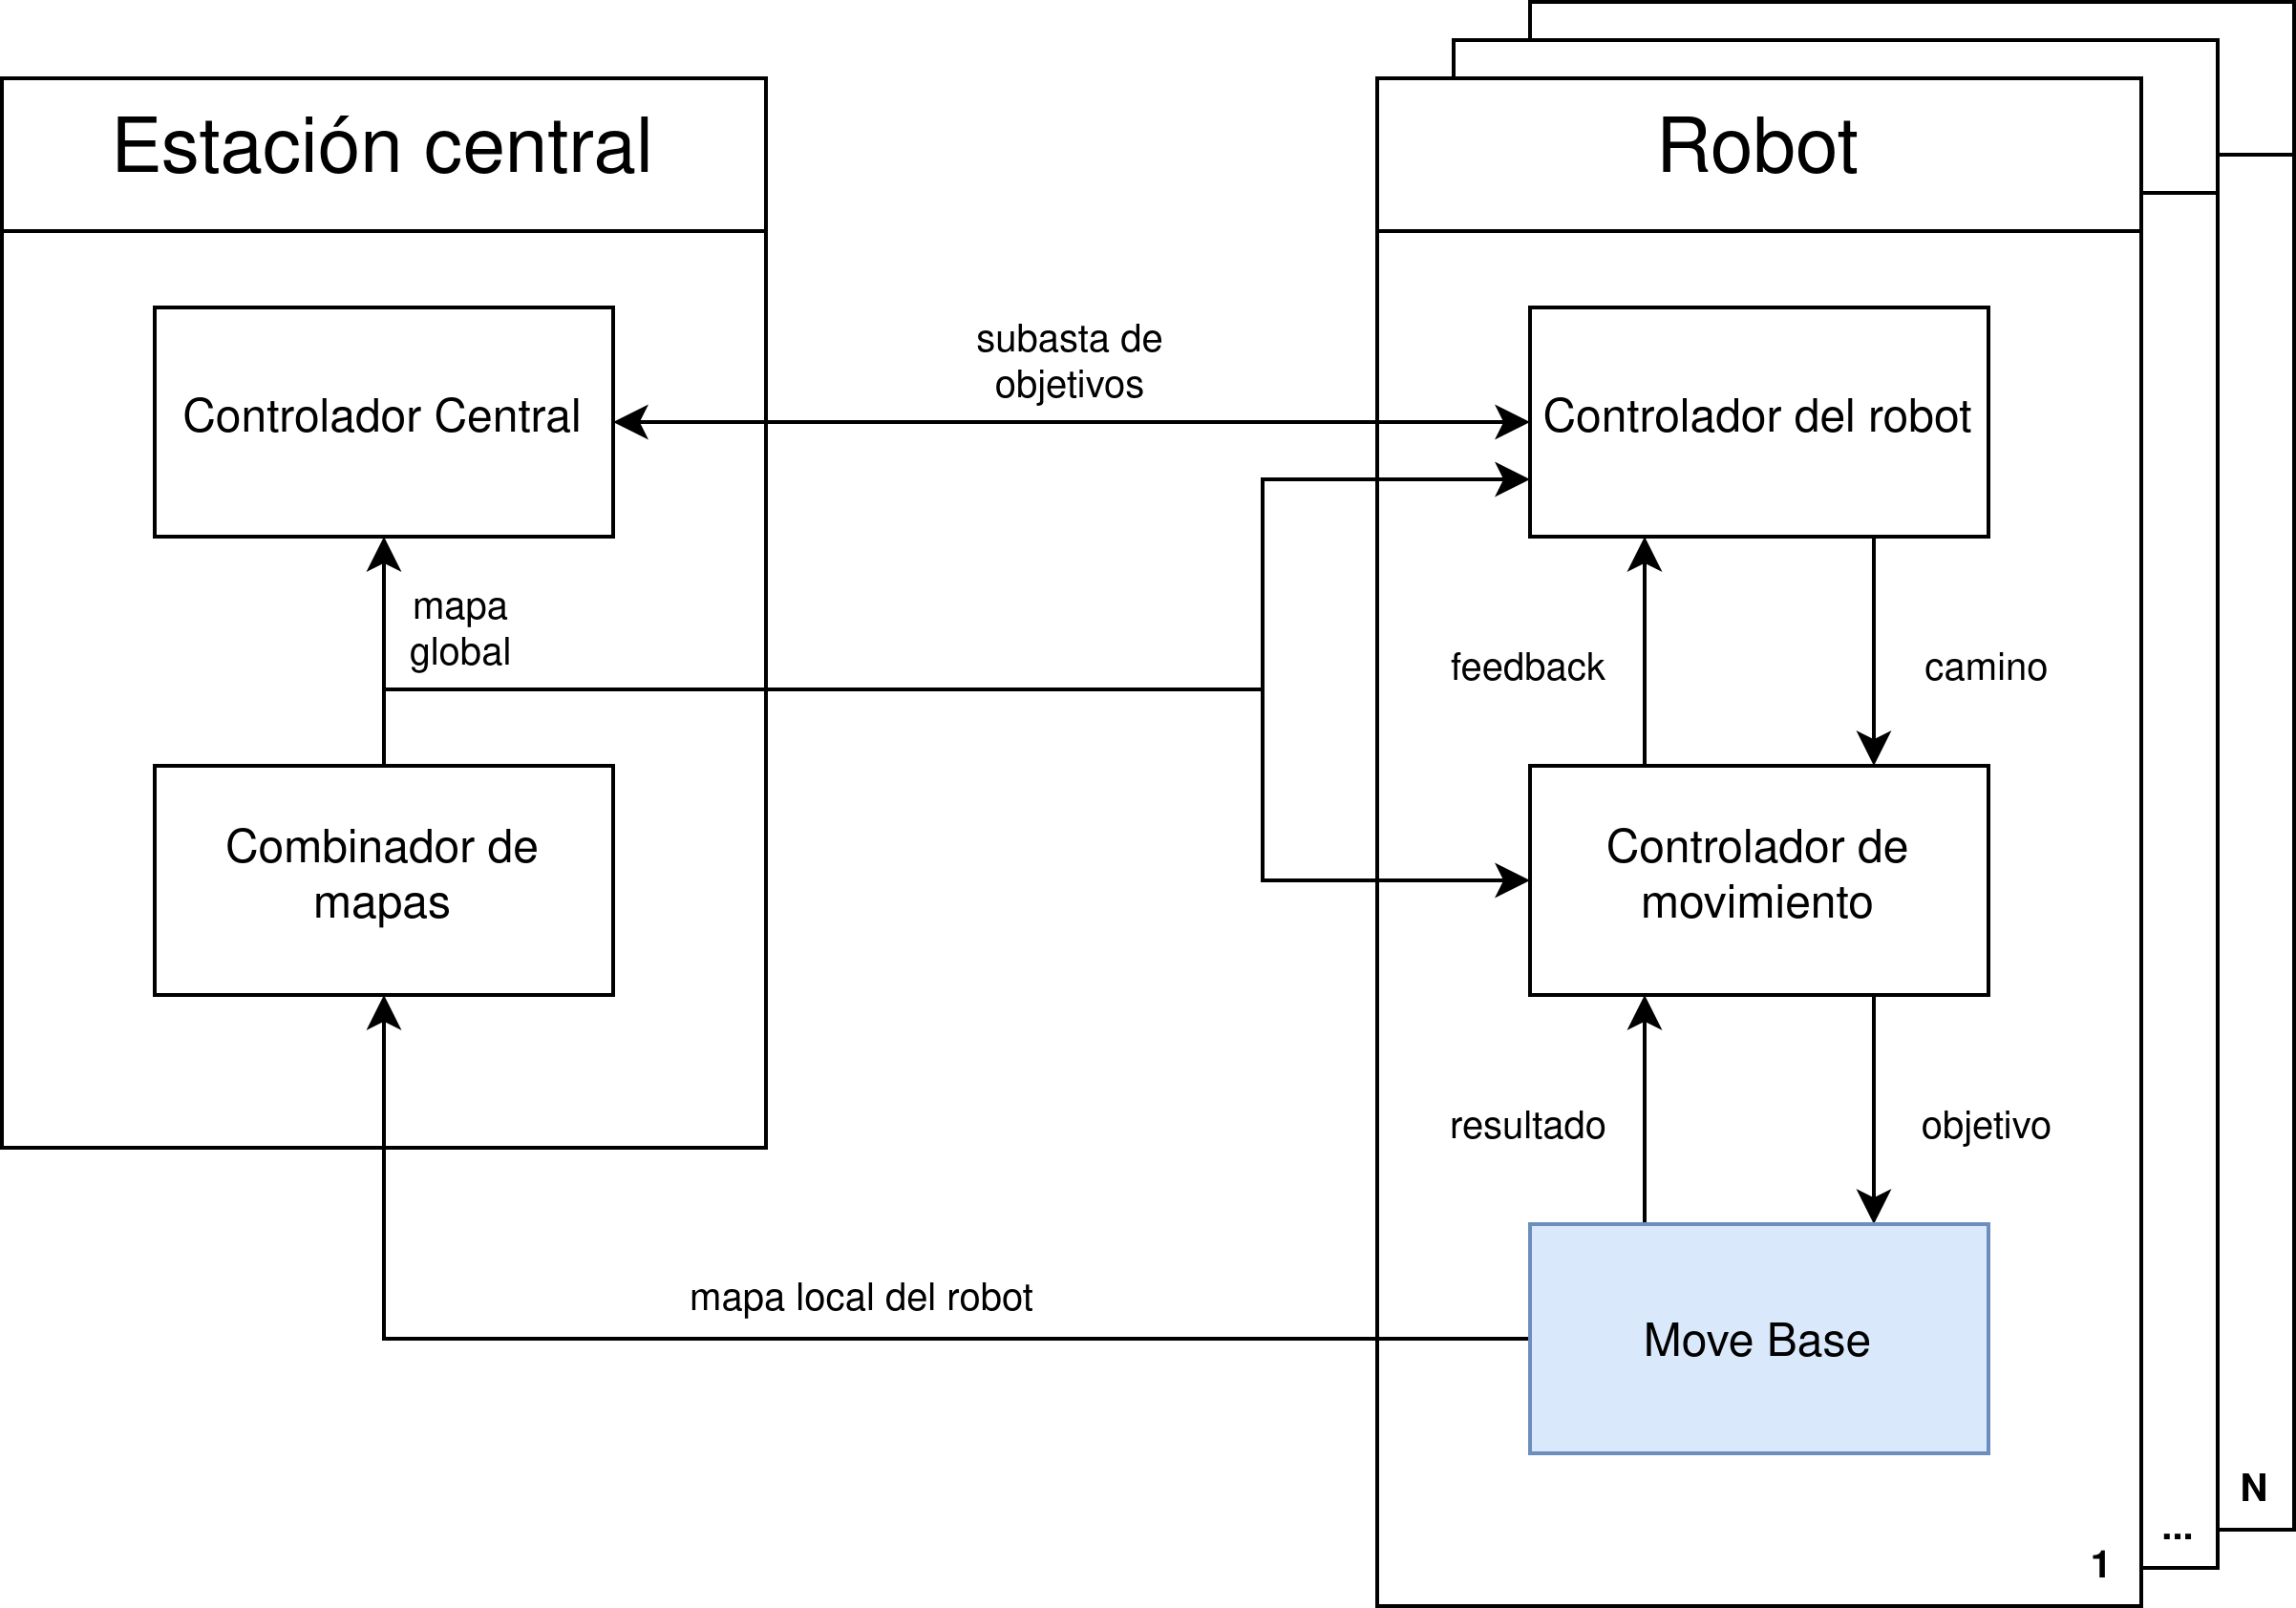
\includegraphics[width=1\linewidth]{imagenes/arquitectura.png}
  \caption[Arquitectura de la solucion propuesta.]{Arquitectura de la solución propuesta. El modulo coloreado con azul es provisto por ROS. Los módulos no coloreados fueron  implementados en esta propuesta.}
  \label{fig:arquitectura}
\end{figure} 

En lo que resta de esta sección se comentará cada modulo, tanto sus tareas y como sus interacciones con el resto de los módulos.

\subsection{Move Base}
El modulo \emph{Move Base} consiste en una instancia del nodo ROS
\emph{move\_base} \cite{ROS-move_base} que provee una interfaz para configurar,
ejecutar y interactuar con el \emph{stack de navegación} de ROS
\cite{ROS-navigation}. 

El stack de navegación de ROS es un conjunto de nodos que tienen como propósito
que un robot pueda navegar el entorno hacia objetivos dentro del mismo. En la
figura \ref{fig:move_base} se muestra un diagrama que repesenta a los nodos que
componen al stack de navegación de ROS y sus interacciones.

\begin{figure}[H]
  \center
  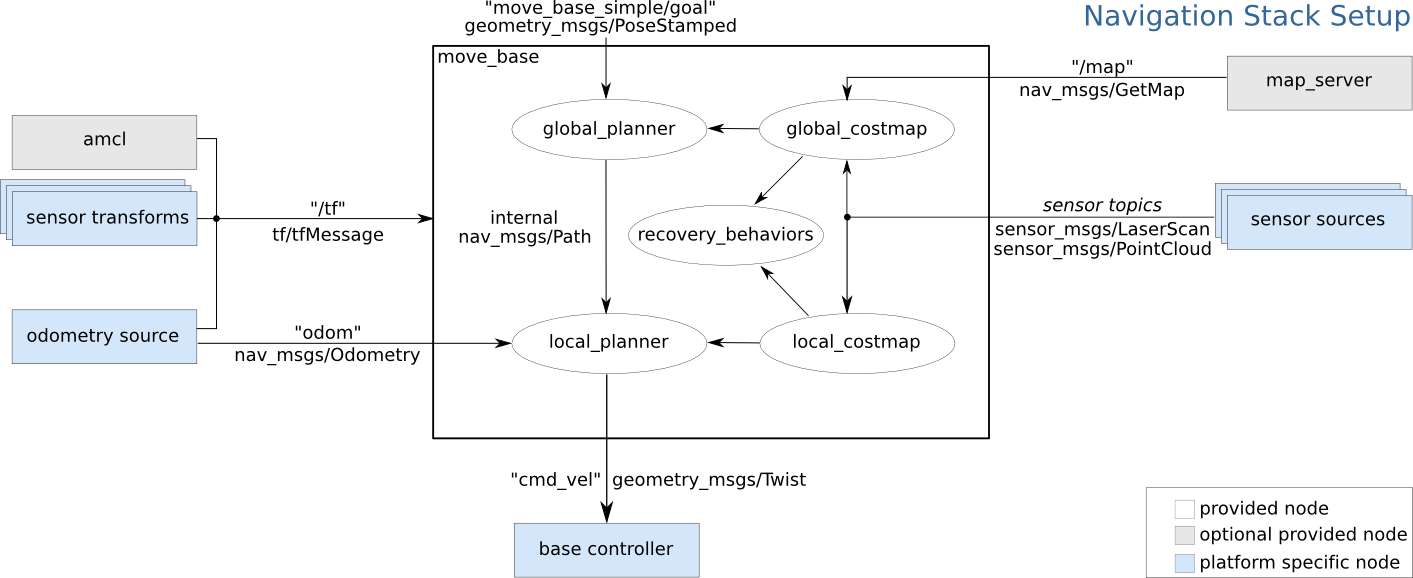
\includegraphics[width=1\linewidth]{imagenes/move_base.png}
  \caption[Arquitectura del stack de navegación de ROS.]{Arquitectura del stack de navegación de ROS. Extraída de \cite{ROS-move_base}.}
  \label{fig:move_base}
\end{figure} 

Cuando se establece un objetivo de navegación este se trasmite al nodo
\emph{global\_planner} este se encarga de generar un plan de alto nivel
consistente de un numero de subobjetivos, que de seguirse en secuencia llevan
al robot al objetivo sin colisiones.

El camino generado por el \emph{global\_planner} es enviado al nodo
\emph{local\_planner} que se encarga de tomar el plan en alto nivel y
traducirlo a la secuencia las velocidades lineales y angulares que un robot
debe tener a lo largo del tiempo para seguir el global. A dicha secuencia de
velocidades se le conoce como plan local.

El stack de navegación permite utilizar distintas implementaciones de
\emph{global\_planner} y \emph{local\_planner}. En el trabajo desarrollado se
hace uso del \emph{global\_planner}\cite{ROS-global_planner} valga la
redundancia llamado \emph{global\_planner} y el \emph{local\_planner} llamado
\emph{teb\_local\_planner}\cite{ROS-teb_local_planner}.

Para generar sus planes tanto \emph{local\_planner} como \emph{global\_planner}
requieren de un mapa, de esto se encargan los nodos \emph{local\_costmap} (mapa
local) y \emph{global\_costmap} (mapa global) respectivamente. Ambos dos son
una instancia de una misma clase de nodo llamada \emph{costmap\_2d}
\cite{ROS-costmap_2d}, que dentro de sus funcionalidades esta la de de
construir una grilla de ocupación a partir de los datos sensoriales provistos
por los robots. Las principales diferencias entre el mapa global y el local son su
tamaño de celda (pequeño en el local y grande en el global), sus dimensiones
del mapa (el mapa global es el mapa completo mientras que el local es solo una
porción) y sus marcos de referencia (el mapa global suele estar fijo, el local se
centra en el robot).

El nodo \emph{recovery\_behaviors} permite ejecutar comportamientos de
recuperación de detectarse que el robot no esta avanzando de forma correcta al
objetivo. Para la solucion desarrollada solo se hace uso del comportamientos de
recuperación que consite en que el robot rote en el lugar.
%en el lugar y forzar que recalculen porciones del mapa.

% El \emph{global\_planner} hace uso de un mapa global, este mapa es provisto por 


% lograr esto cuando se establece un objetivo de navegación,


% de permitir que un robot pueda mover que a partir de información sobre la ubicación, sensores del robot, v 


\subsection{Combinador de mapas}
El modulo \emph{Combinador de mapas} es el encargado de mantener el mapa del entorno
explorado. Este recibe las actualizaciónes de los mapas globales que son
generados por el nodo \emph{global\_costmap} del stack de navegacion de cada
robot y las combina en un unico mapa que contenga toda la información
recopilada del entorno. Cuando el mapa combinado global se actualiza este
retrasmite lo actualizado a diversos componentes del sistema (ver figura
\ref{fig:arquitectura}) que utlizan el mapa del entorno explorado para llevar a
cabo alguna de sus tareas. 

\subsection{Controlador central}

El modulo \emph{Controlador central} lleva a cabo la identificacion de objetivos, es decir detectar en
el mapa actual los potenciales objetivos de exploracion. 

A su vez es el principal responsable de realizar la asignacion de objetivos.
Específicamente la asignacion de objetivos consiste en una subasta en la cual
este modulo actua como subastador. La subasta se puede resumir de la siguiente
manera, los objetivos de exploracion identificados son transmitidos desde el
\emph{controlador central} a los robots los cuales valuan a dichos objetivos segun que
tan conveniente les es llegar a ellos. Los robots envian sus valuaciones a la
central la cual aplica una algorimo para determinar que objetivo le corresponde
a cada robot y posteriormente le informa a cada robot que objetivo le
corresponde.

% tiene el
% siguiente funciona en la cual  de objetivos consite en tomar los objetivos
% identificados y coordinar

% La prinicpal es la de llevar a cabo la identificación de tareas y ser el 

% e encarga de coordinar las subastas de segmentos, es decir, genera la
% información necesaria para esta, decide cuando comienza la subasta y cuando
% termina el plazo para ofertar, computa los resultados y se encarga de las
% comunicaciones necesarias para llevarla a cabo.

\subsection{Controlador de movimiento}
El modulo \emph{Contrador de movimiento} es como su nombre lo indica el modulo
que se encarga de controlar el movimiento del robot. Específicamente recibe
caminos compuesto por celdas de la grilla de ocupacion que en secuencia llevan
a un objetivo de exploracion, y se encarga de ir enviando objetivos de
navegacion al modulo \emph{Move Base} para que el camino sea ejecutado de forma
rapida evitando maniobras innecesarias.

Tambien lleva a cabo una capa superior de comportamientos de recuperacion
extendiendo los provistos por el modulo \emph{Move Base}.

Indica al \emph{Controlador del robot} si se completo el camino con exito, o
existe algun problema.

\subsection{Controlador del robot}
El \emph{Controlador del robot} es el modulo que se encarga de valuar los
objetivos cuando ocurre una subasta. A su vez se encarga de procesar las
asignaciones de objetivos determinadno el camino que lleva al objetivo y
enviandolo al modulo \emph{Controlador de movimiento}. 

Tambien es responsable por solicitar el inicio de una subasta al
\emph{Controlado central} cuando el \emph{Controlador de moviemiento} indica el
exito o el fracaso en seguir el camino asignado.

% Tambien pide la subasta.\todo{explicar mejor}

% \section{Ciclo de robot}

% \section{Ciclo de la central}
\section{Definiciones}
\subsection{Grillas de ocupacion}
En el contexto de este trabajo se utlizara las siguientes definiciones referentes a
grillas de ocupacion, introducidas en la seccion \ref{subsec:mapas}.

El conjunto $C\subseteq R^2$ esta conformado de los centros de cada celda de la
grilla de ocupacion. Las celdas se repreresentan segun sus centros y viceversa
sin ambigüedad, por lo tanto en lo que resta de este informe se usaran ambos
terminos de forma indistinta.

Se dice que cada celda $c\in C$ tiene asociada una probabilidad $P(c|m(1:k))$
de estar ocupada, donde $m(1:k)$ es el conjunto de medidas resultantes de algun
sensor desde el comienzo de la exploarcion.

La funcion $e : C \rightarrow E$ dado un centro de celda, devuelve uno de los
tres estados posibles $E=\{libre, ocupado, desconocido\}$ segun la probabilidad
asociada a $c$. En el contexto de este proyecto la funcion $e$ se define segun
(\ref{eq:estado}).
\begin{equation} 
  e(c)= 
  \left \{ 
    \begin{aligned}
       libre       &\ \ \ \text{ si}& P(c|m(1:k)) < 0.5 \\
       desconocido &\ \ \ \text{ si}& P(c|m(1:k)) = 0.5 \\
       ocupado     &\ \ \ \text{ si}& P(c|m(1:k)) > 0.5
    \end{aligned}
  \right .
  \label{eq:estado}
\end{equation}

La funcion $ady : C \rightarrow P(C)$ dada una celda devuelve el conjunto de
celdas adyacentes a la misma. La definicion de $ady$ utlizada en el contexto de
este proyecto se presenta en (\ref{eq:vecinos}) donde $n_1, n_2, ..., n_8$ se
corresponden a vecinos diagonales y horizontales de $c$ segun se muestran en la
figura \ref{fig:vecinos}.

\begin{equation} 
 ady(c)=\{n_i : 1\leq i \leq 8, n_i \in C\}
 \label{eq:vecinos}
\end{equation} 

\begin{figure}[H]
  \center
  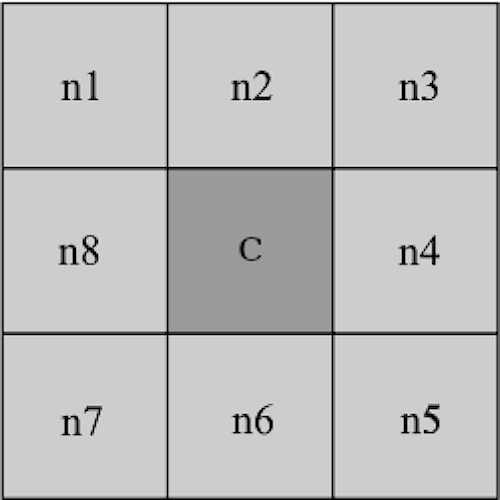
\includegraphics[width=0.3\linewidth]{imagenes/vecinosSharp.png}
  \caption[Vecinos de una celda en una grilla de ocupación.]{Vecinos de una celda en una grilla de ocupación.}
  \label{fig:vecinos}
\end{figure} 

Notar que la relacion de adyacencia es simetrica por lo que $c_1 \in ady(c_2) \Leftrightarrow c_2 \in ady(c_1)$.
% This map is obtained from the occupancy probability grid by a simple clipping operation with a threshold of 0.5. The gray areas of the maximum-likelihood map correspond to cells that have not been sensed by the robot.

\subsection{Componentes conexas} \label{subsec:CompComp}
Una descomposicion en componentes conexas de un conjunto de
celdas $C$ es un conjunto $CC\in P(C)$ compuesto por $N$ conjuntos $C_i$ con
$i\in[1,N]$ tales que:
\begin{itemize}
  \item $\bigcup_{i=1}^{N}C_i = C$ 
  \item Para todo $i,j \in [1,N]$ $C_i\cap C_j = \emptyset$
  \item Para todo $i \in [1,N]$, para todo par $c_1,c_2 \in C_i$ se cumple que $c_1 \in ady(c_2)$.\todo{arrglar, seria hay camnio en $C_i$}
  \item No existen $i,j \in [1,N]$ tales que existan $c_1 \in C_i$ y $c_2 \in C_j$ que cumplan con $c_1 \in ady(c_2)$ 
\end{itemize}

Un ejemplo de una descomposicion en componentes conexas se muestra en la figura \ref{fig:fronterasCompCon}.

\begin{figure}[H]
  \centering
  \subfloat[Las celdas pertenecientes a $C$ se marcan con azul.]{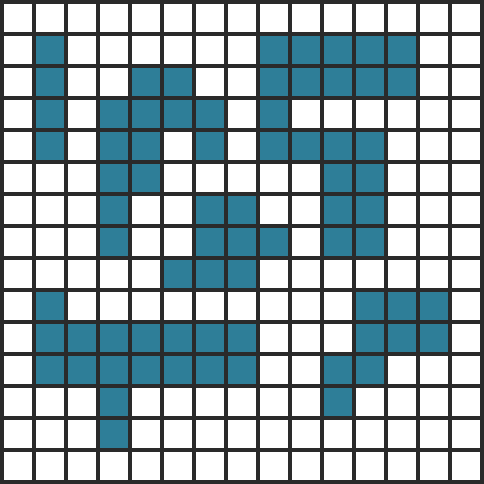
\includegraphics[clip=true, width=0.40\linewidth]{imagenes/compCon/a.png}}
  \qquad
  \subfloat[Cada componente conexa de $C$ se contornea con rojo.]{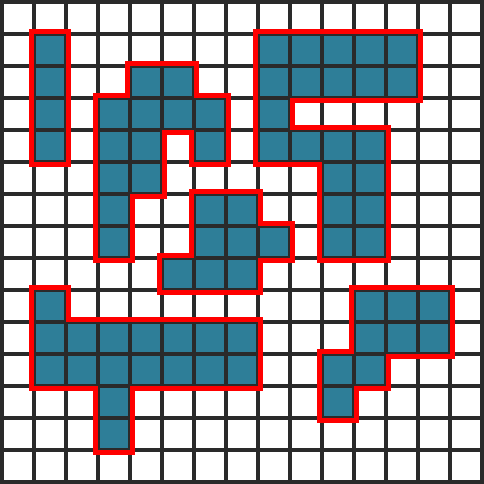
\includegraphics[clip=true, width=0.40\linewidth]{imagenes/compCon/b2.png}}

  \caption{Descompocicion en componentes conexas.}\label{fig:descCompCon}
\end{figure}

Es posible obtener las compnentes conexas de un conjunto cualquiera de
celdas $C$ con el algoritmo \ref{alg:compcon}.

\begin{algorithm}[H]
\SetAlgoLined
  \SetKwInOut{Input}{Entrada}
  \Input{$C$}
  $restantes := C$ \\
  $CC := \emptyset$ \\
  $pila :=$ Pila vacia \\
  $i := 1$ \\
  \While{ $\neg restantes.vacia()$ } {
    $C_i := \emptyset $ \\
    $c :=$ elemento arbitrario de $Restantes$ \\

    % \tcp{DFS desde $c$ agregando las celdas visitadas a la componente conexa $C_i$}

    $C_i :=  C_i \cup \{c\}$ \\
    $restantes := restantes - \{c\}$ \\
    $pila.apilar(c)$ \\
    \While { $\neg pila.vacia()$ } {
      $c := pila.desapilar()$ \\
      \For{ $cA \in ady(c)$ } {
        \If{ $cA \in restantes$ } {
          $C_i :=  C_i \cup \{c\}$ \\
          $restantes := restantes - \{c\}$ \\
          $pila.apilar(c)$ \\
        }
      }
    }
    $CC := CC \cup C_i$ \\
    $i := i + 1$ \\
  }
  \Return $CC$ 

  \caption{Descomposicion en componentes conexas de $C$}
  \label{alg:compcon}
\end{algorithm}

Este algoritmo se resume en elegir una celda $c\in C$ que no este aun en una
componente conexa (linea 6), aplicar un \emph{depth-first search} (DFS)
partiendo $c$ agregado todas las celdas recorridas a una misma componente
conexa (lineas 7-19). Repetir dicho procedimiento hasta que todas las celdas
pertenezcan a alguna componente conexa (linea 4). Este algormitmo es analogo al
que esta presente en \cite{hopcroft1973algorithm}.

\section{Identificación de objetivos}
El problema de identificación de objetivos consiste en determinar los puntos
del espacio a los cuales es conveniente enviar robots para recolectar nueva
informacion sobre el entorno explorado. Estos puntos son los llamdos objetivos
de exploración (seccion \ref{sec:exploracion}). 
% En el contexto del trabajo desarrollado al utlizarse una grilla de ocupacion
% como mapa los 
% se hablara de celdas en lugar de puntos, existiendo una correspondencia entre
% cada celda y un unico punto en el espacio, su centro.

\subsection{Fronteras}
En \cite{yamauchi1998frontier} se propone que los lugares que permiten
recolectar la mayor cantidad de nueva informacion sobre el entorno son las
fronteras entre el espacio conocido y desconocido. Y que por lo tanto dichas
fornteras deben ser los objetivos de exploración.
Al utlizar una grilla de ocupacion como mapa, las fronteras se definen como las
celdas cuyo estado asociado es $libre$ y son adyacentes a una celda cuyo estado
asociado es $desconocido$ (figura \ref{fig:fronteras}).
Por lo tanto segun Yamauchi los objetivos de exploración seran las celdas
fronteras $F$ segun se definen en (\ref{eq:fronteras}).
\begin{equation} 
  F = \{ c \in C : e(c) = libre, \exists n \in ady(c), e(n) = desconocido  \}
  \label{eq:fronteras}
\end{equation}

\subsection{Simplificacion de Fronteras basada en K-Means}
En \cite{amorin2019novel} se argumenta que tratar todas las celdas fronteras
como objetivos de exploración diferentes podría ser computacionalmente
prohibitivo. Por lo tanto, para reducir el costo computacional, se intenta
reducir los objetivos de exploración a las celdas frontera mas representativas,
a las cuales se denominaran como fronteras significativas.

Para determinar las fronteras significativas, primero, las celdas fronteras $F$
se descomponen en sus componentes conexas $\mli{FC}=\{F_1,F_2,...F_N\}$
(seccion \ref{subsec:CompComp}), un ejemplo de este tipo de descomposicion se
puede ver en la figura \ref{fig:fronterasCompCon}.

Luego se determinan las fronteras significativas $\mli{FS}_i$ de cada
componente conexa $F_i\in \mli{FC}$. Esto se hace agrupando las fronteras de
$F_i$ con el algoritmo K-Means \cite{macqueen1967some}, y determinando una
frontera significativa por cada una de las $k$ agrupaciones, la
frontera mas cercana de $F_i$ al centroide de la agrupacion (una arbitraria de
las mas cercanas en el caso de que exista mas de una). Un ejemplo de las
fronteras significativas  $\mli{FS} = \bigcup_{i=1}^N \mli{FS_i}$ obtenidas con
este metodo se muestra en la figura \ref{fig:fronterasSig}.

El $k$ utilizado para ejecutar K-Means es el minimo que logra que para toda
frontera $f\in F_i$ existe $\mli{fs} \in FS_i$ tal que $d_{\mli{fs}}(f) \leq
rango$ siendo $rango$ el alcance de los sensores del robot. Es decir, el
conjunto de fronteras significativas $\mli{FS}_i \subset F_i$ cumple con que
cada frontera esta dentro del rango del sensado de alguna frontera
significativa, cuando esto se cumple se dice que $\mli{FS}_i$ cubre a $F_i$, o
que $FS_i$ logra el cubrimiento. En la figura \ref{fig:fronterasSigCub} se
puede ver como las fronteras significativas obtenidas $FS$ logran el
cubrimiento, ya que todas los centros de las fronteras $F$ estan contenidos en
las circunferencias de radio $rango$ centradas en las fronteras significativas
$FS$.

Para encontrar el minimo $k$ con las que se logra un $\mli{FS}_i$ que cubra a
$F_i$, se parte con $k=1$, si el resultado no logra cubrir incrementa $k$ y se
repite el proceso.


\begin{figure}[H]
  \centering
  \subfloat[Se identifican las frotneras,  marcadas con amarillo.]{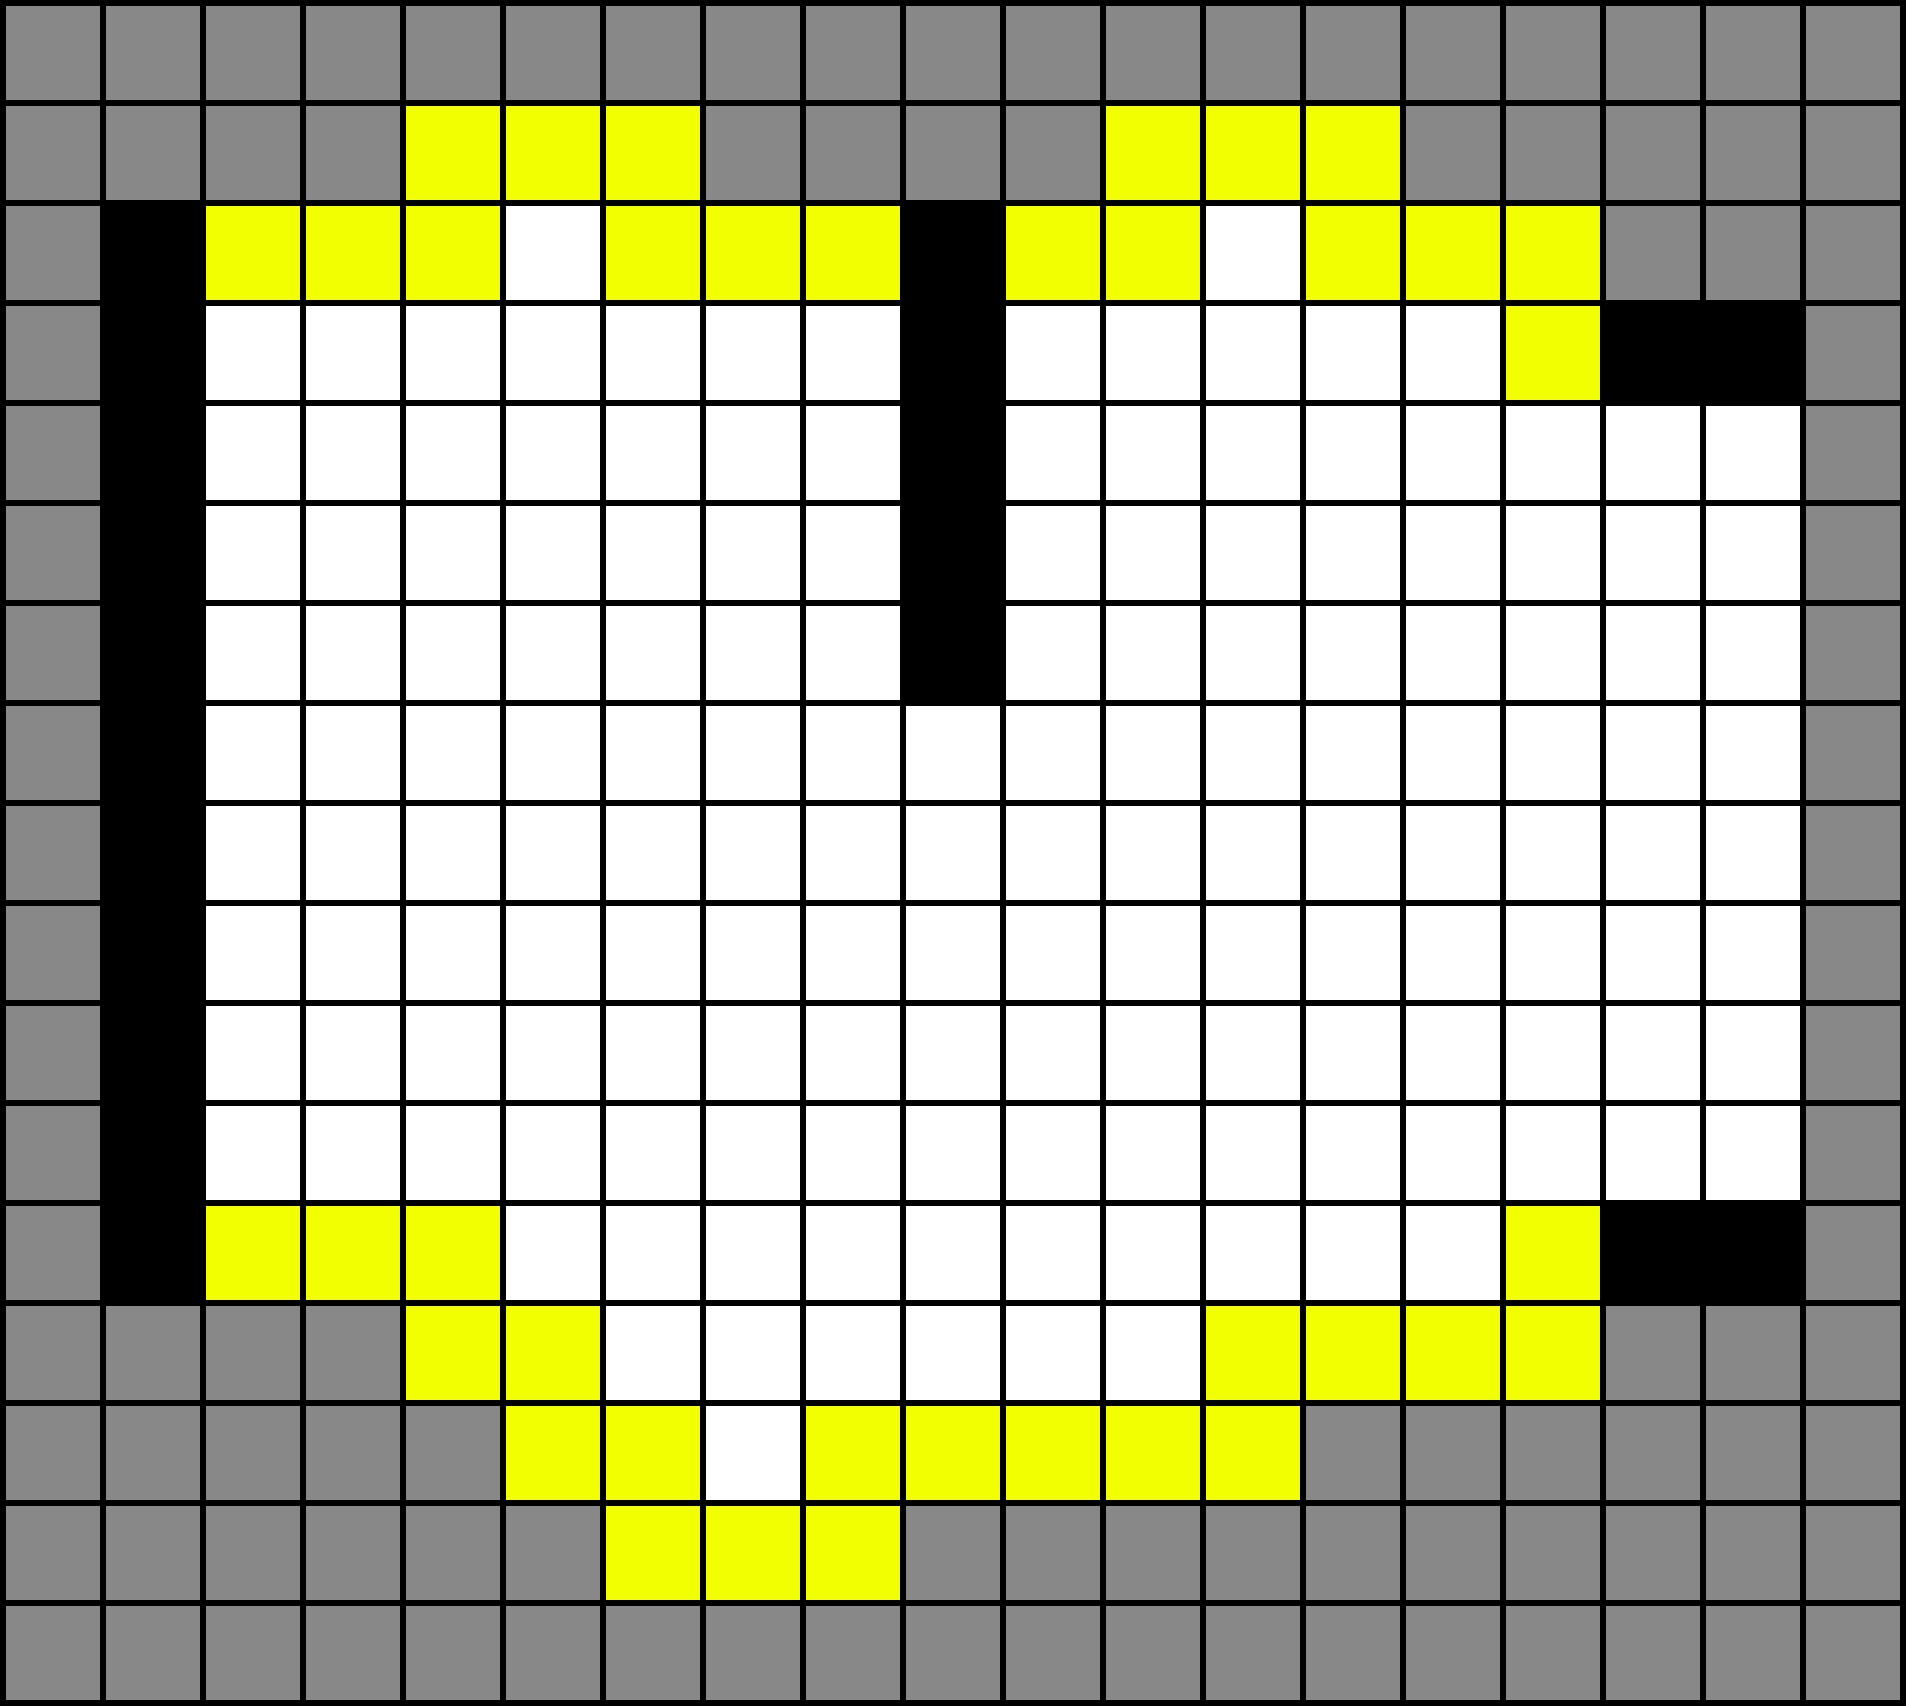
\includegraphics[clip=true, width=0.40\linewidth]{imagenes/fronterasSig/a.png}\label{fig:fronteras}}
  \qquad
  \subfloat[Descompocicion de las fronteras en componentes conexas, cada componente conexa se indica con un color distinto.]{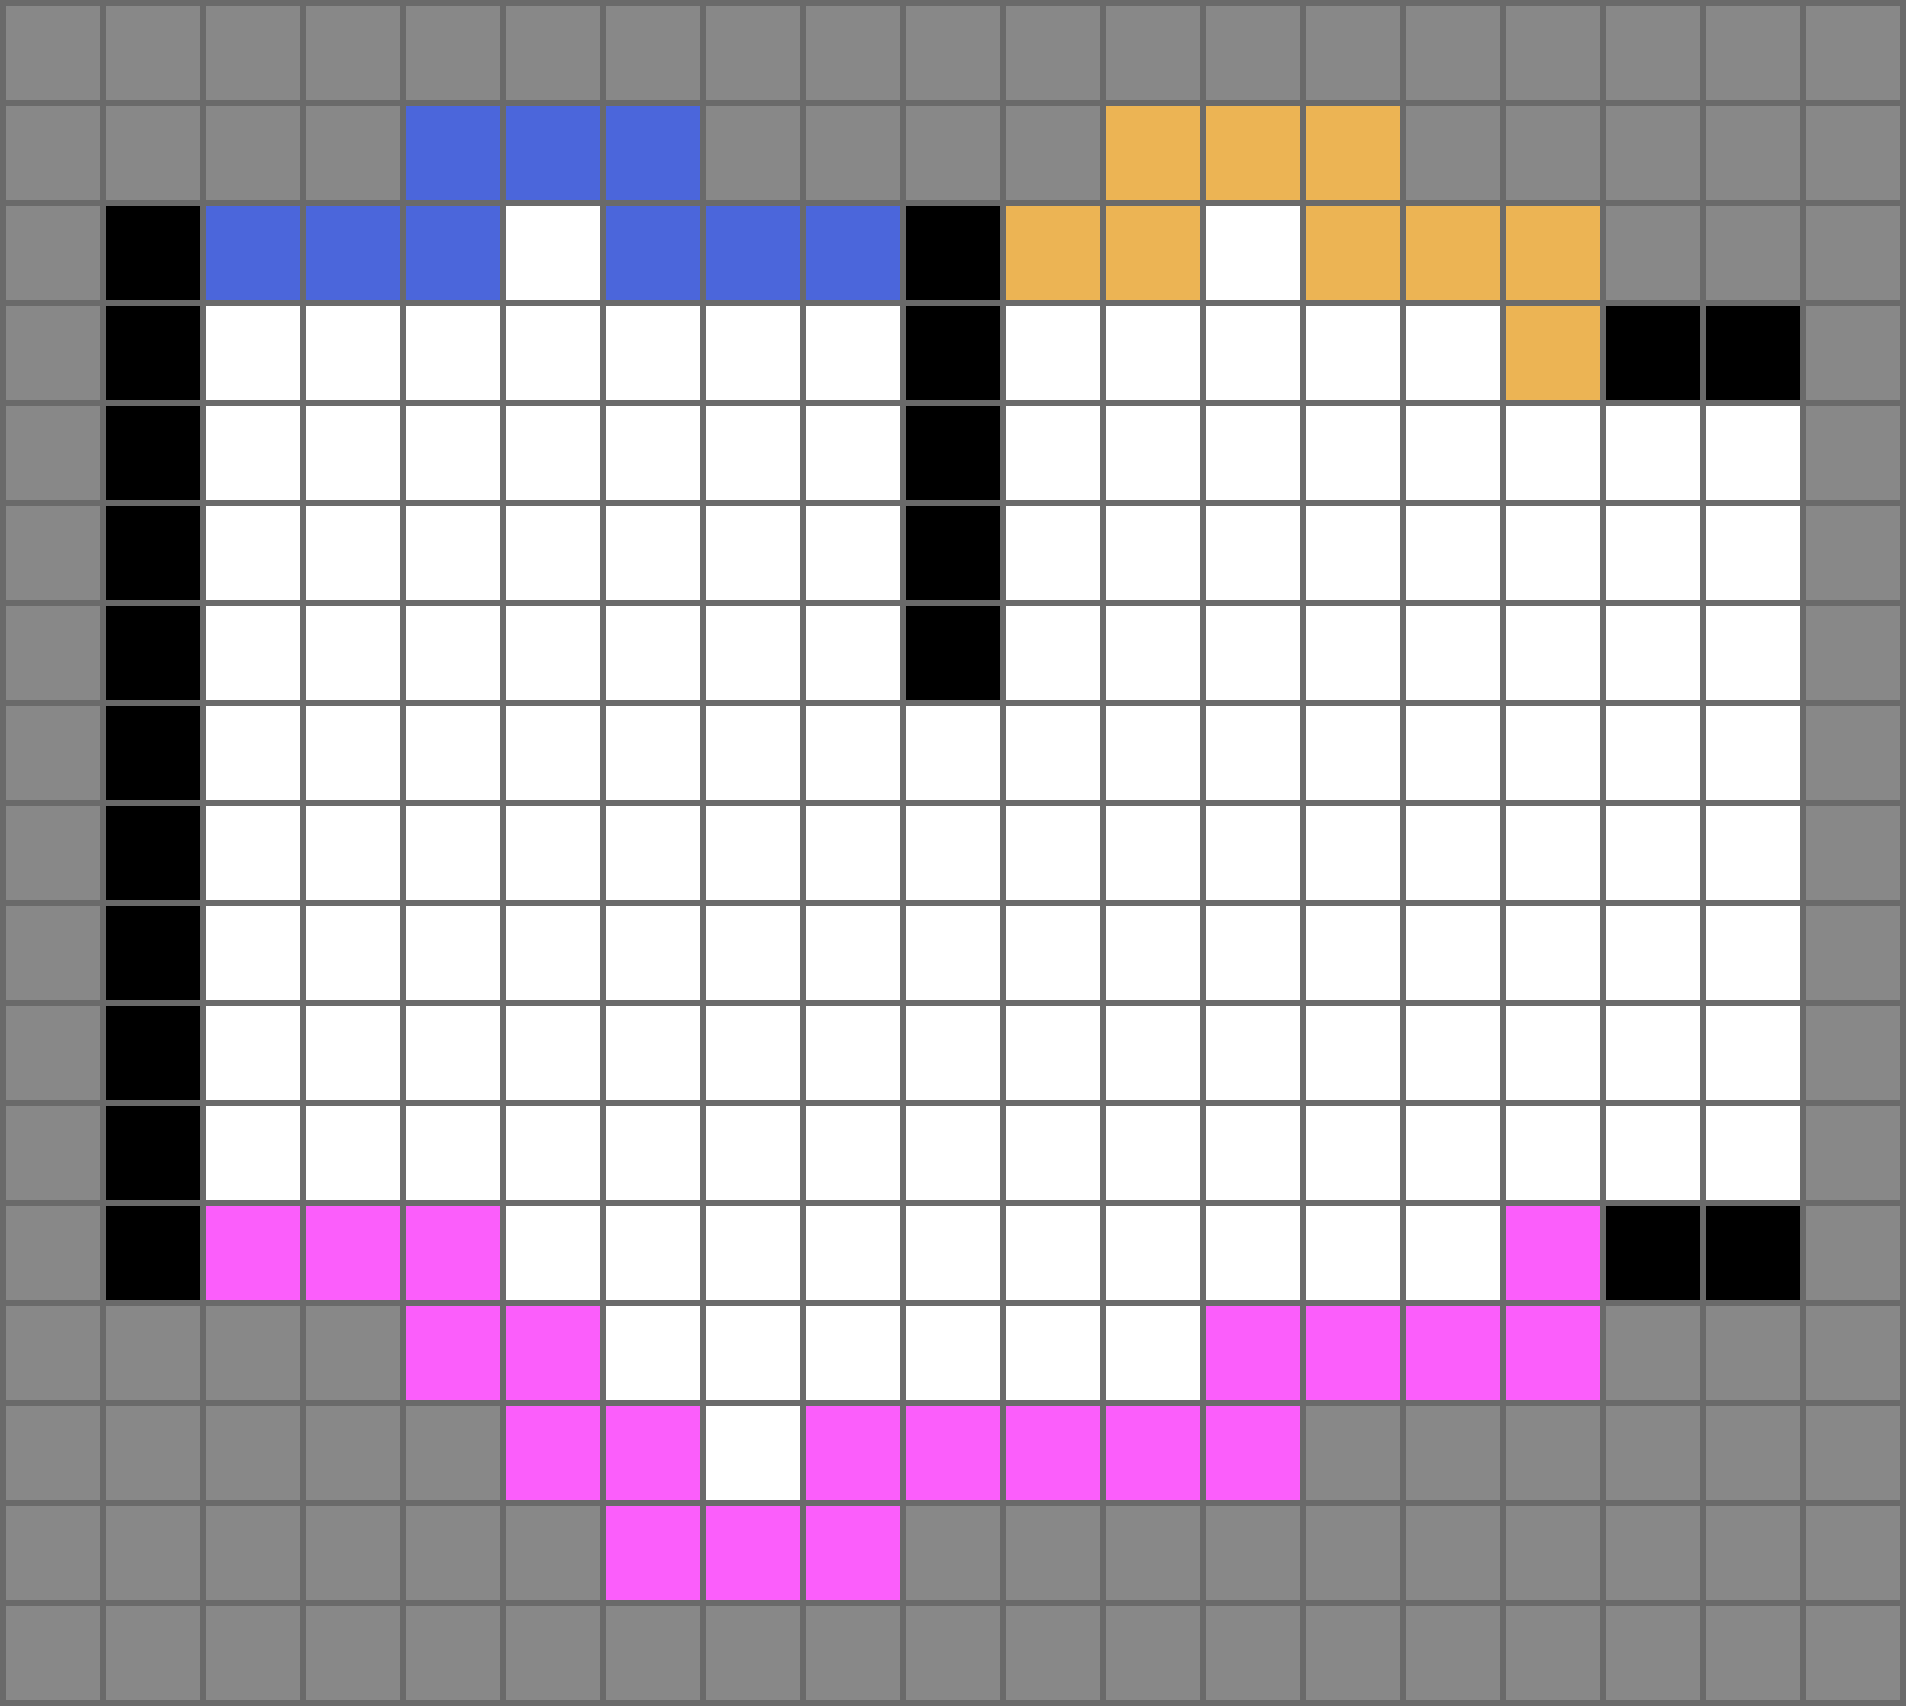
\includegraphics[clip=true, width=0.40\linewidth]{imagenes/fronterasSig/b.png}\label{fig:fronterasCompCon}}
  \qquad
  \subfloat[Fronteras significativas (indicadas con verde) de cada componente conexa.]{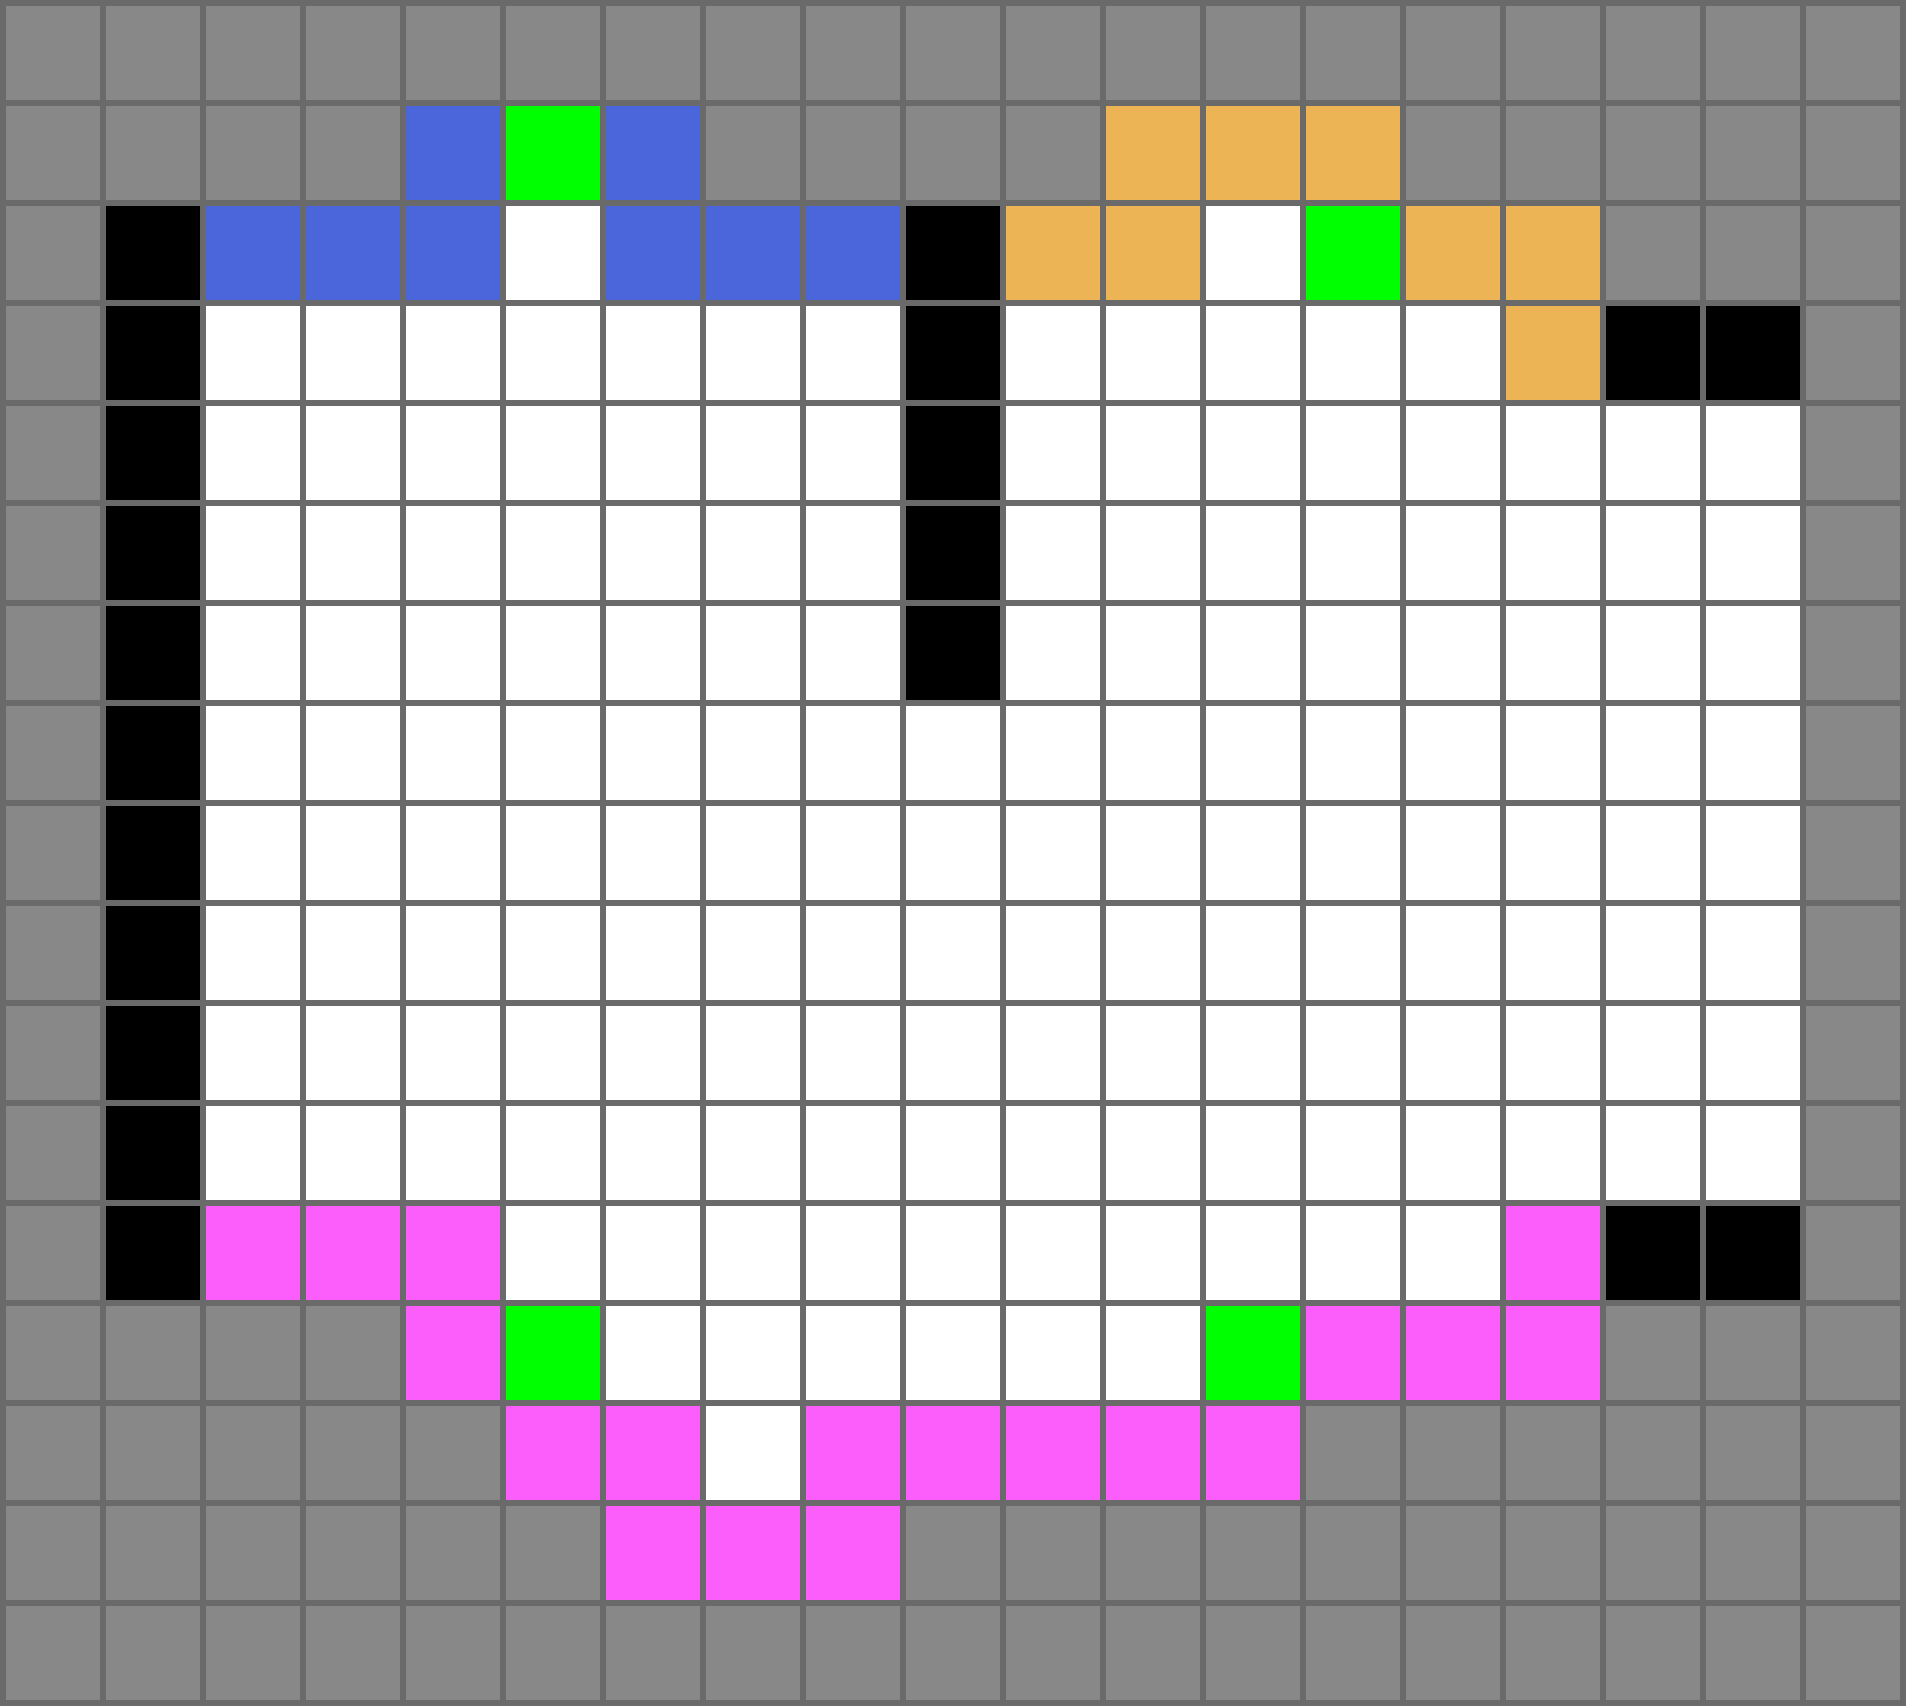
\includegraphics[clip=true, width=0.40\linewidth]{imagenes/fronterasSig/c.png}\label{fig:fronterasSig}}
  \qquad
  \subfloat[Se logra el cubrimiento.]{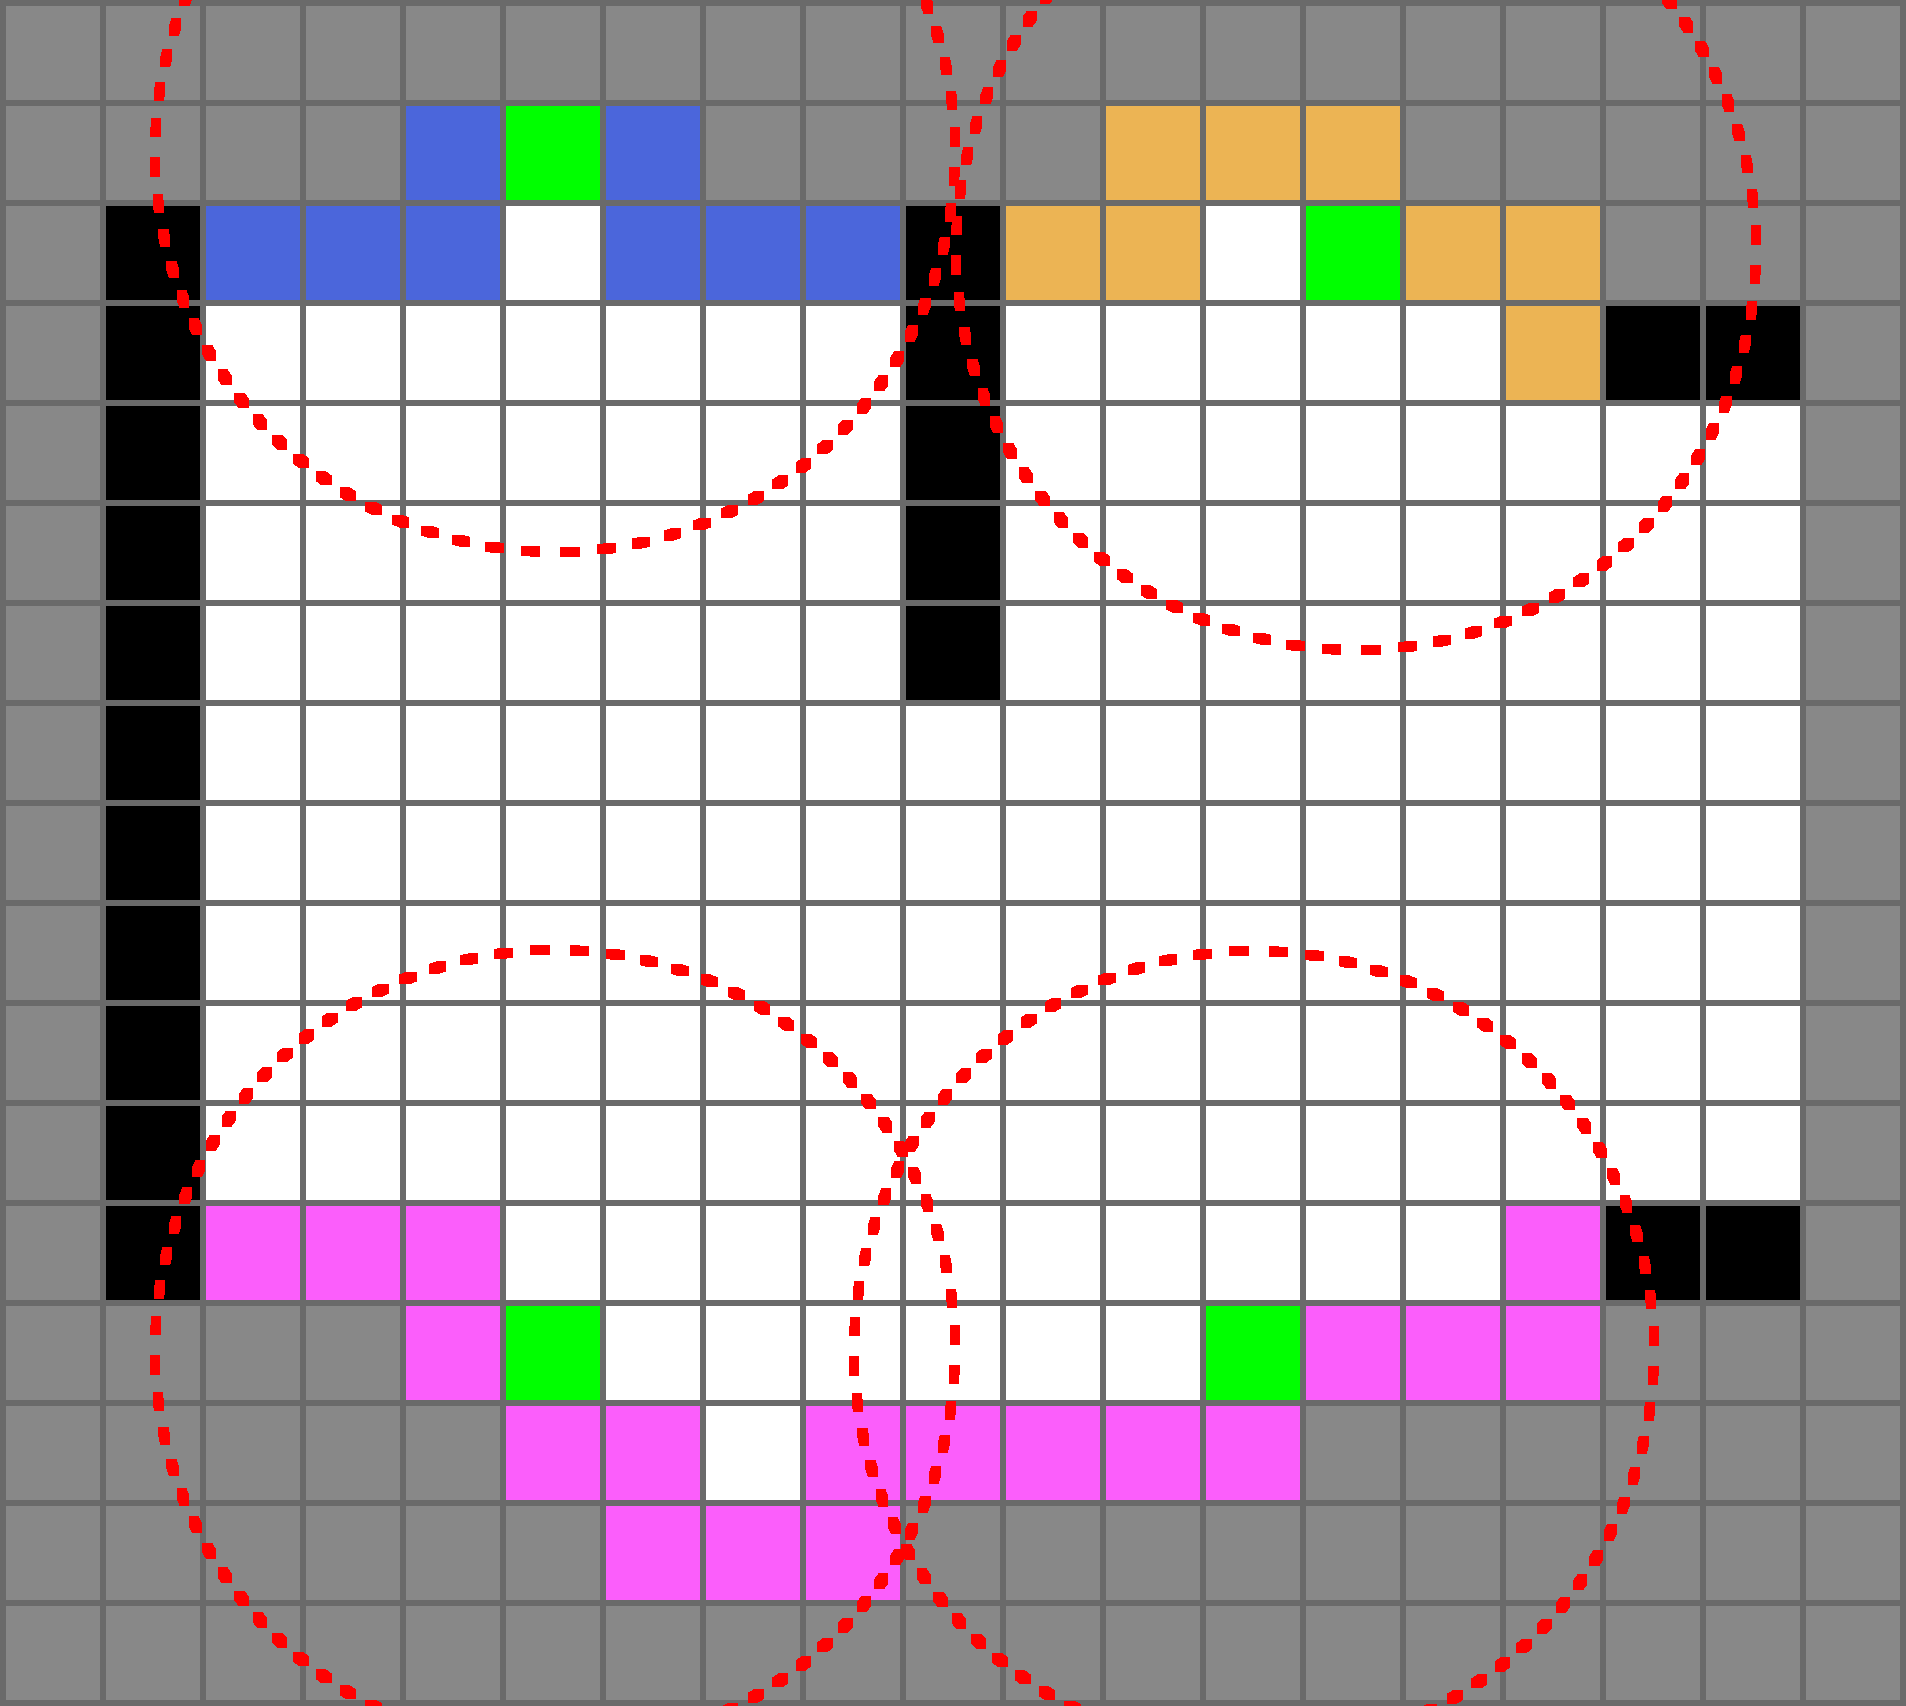
\includegraphics[clip=true, width=0.40\linewidth]{imagenes/fronterasSig/d.png}\label{fig:fronterasSigCub}}

  \caption[Proceso de simplificacion de fronteras según K-Means.]{Proceso de
    simplificacion de fronteras según K-Means. Las circunferencias rojas
    centradas en las fronteas significativas tienen radio $rango=4$ (largos de celda) indicando su
    cubrimiento.
  \cite{Amorin2019}.}\label{fig:ejemploFrontSig}
  % \caption[Proceso de simplificacion de fronteras según K-Means.]{Proceso de simplificacion de fronteras según K-Means. Cada figura corresponde a un mismo entorno parcialmente explorado, representado con una grilla, donde las celdas blancas son libres, las negras ocupadas, y para las grises se desconoce su estado. Basada en figuras de \cite{Amorin2019}.}\label{fig:ejemploFrontSig}
\end{figure}

% En la seccion anterior se presento un metodo que soluciona el siguiente
% problema. Dado un conjunto de  la descomposicion en componentes conexas de
% $F$, $\mli{FC}=\{F_1,F_2,...F_N\}$ se obteniene como salida el conjunto
% $\mli{FS} = \bigcup_{i=1}^N \mli{FS_i}$ que cumple con la restriccion de que
% para todo $i \in [1,N]$ $\mli{FS}_i$ cubre a $F_i$.

El problema descrito hasta el momento se puede resumir en el de  dado un
conjunto de fornteras $F$, obtener un conjunto de fornteras significativas
$\mli{FS}$ que cumplen con la restriccion de que $\mli{FS}$ cubre a $F$.
Recordando que el proposito de usar $\mli{FS}$ como objetivos de exploracion en
lugar de usar $F$ es reducir los objetivos de exploracion entoces es natural
pensar que la soluciones optimas reducen al minimo el $\mli{FS}$ resultante,
mientras mantienen la restriccion de cubrimiento.

% Analizando la restriccion de cubrimiento, se puede ver que un indicador de que
% una solucion es suboptima es que varias celdas $\mli{FS}$ se concentren,
% solapandose las circunferencias de radio $rango$ centradas en ellas. Por
% ejemplo 

Dado esto es posible ver que en el ejemplo presentado en
\ref{fig:ejemploFSKMMal} el resultado obtenido por el metodo presentado en esta
seccion no es optimo ya que existen fronteras significativas innecesarias para
el cubrimiento. 

\begin{figure}[H]
  \centering
  \subfloat[Fronteras significativas obtenidas segun el metodo basado en K-Means.]{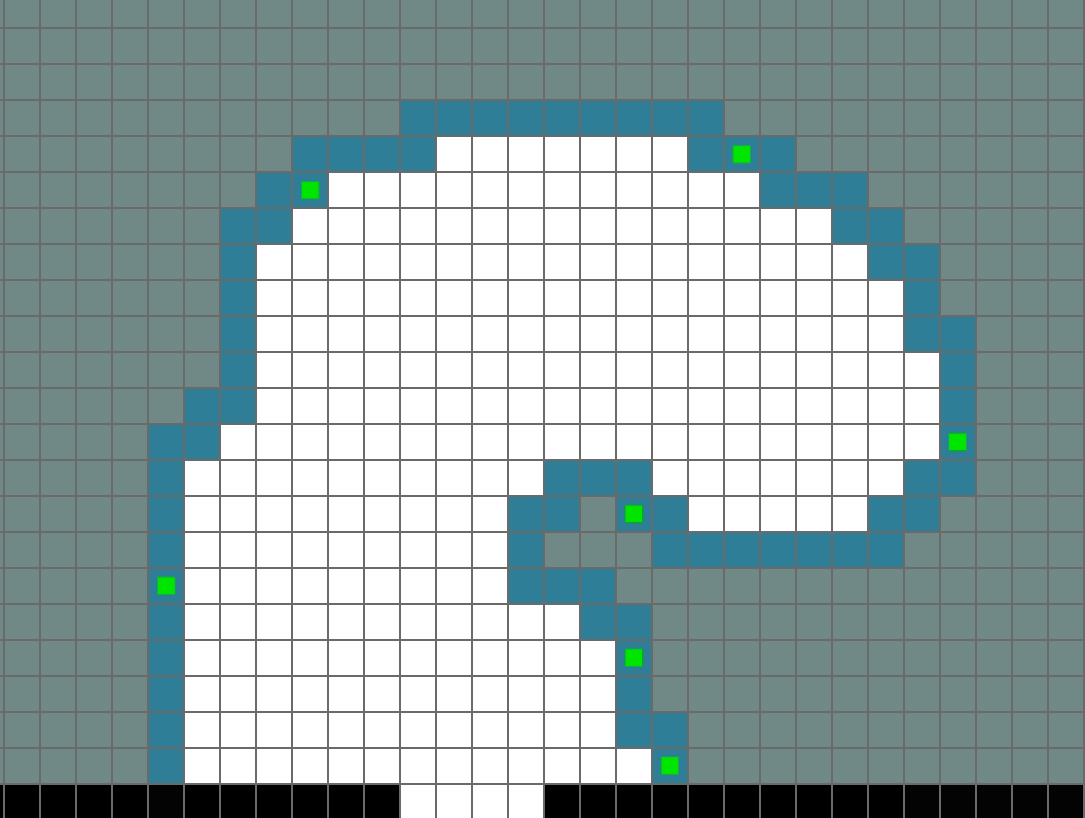
\includegraphics[clip=true, width=0.40\linewidth]{imagenes/fronterasigKMMal/caso1/a_sin_circ.png}}
  \qquad
  \subfloat[Dos de las fronteras significativas de la parte inferior derecha de (a) no son necesarias para lograr el cubrimiento.]{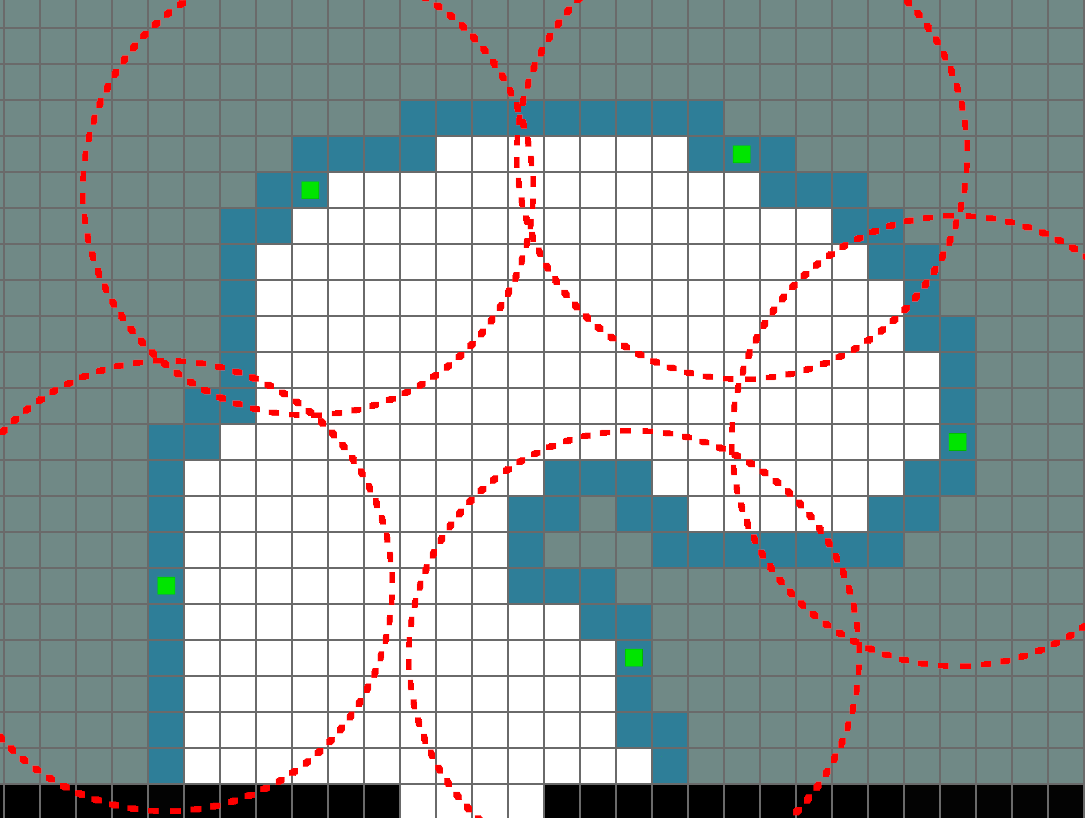
\includegraphics[clip=true, width=0.40\linewidth]{imagenes/fronterasigKMMal/caso1/b.png}}

  \caption[Simplificacion de fronteras suboptima resultante del metodo basado en K-Means.]{Simplificacion de fronteras suboptima resultante del metodo basado en K-Means. Las fronteras de $F_i$ se indican con azul, las fornteras significativas con verde y las
    circunferencias rojas centradas en estas tienen radio $rango=5.6$ (largos de celda) indicando su
    cubrimiento. Extraída de implementacion desarrollada\footnotemark.}\label{fig:ejemploFSKMMal}
\end{figure}
\footnotetext{Podria indicar el bag y el seg}

Resultados suboptimos similares se experimentan de forma consistente %al aplicarse la simplficacion 
sobre componentes conexas con forma serpenteante\todo{no se si este termino se entiende, me es dificil explicarlo bien, con forma de S?},
asimetricas y lo suficientemente extensas como para requerir mas de 4
fornteras significativas para su cubrimiento, 
%con un largo mayor a $rango*8$ 
% \todo[inline]{se entiende la idea del largo aplicada a esto? Creo que puede
% quedar claro mirando la foto pero tengo mis dudas. La idea en realidad seria
% decir que la solucion no es lo suficientemente simple, por ejemplo si con 1
% sola frontera sig ya se cubre todo entonces no va haber problema sin importar
% que tan serpenteante o asimetrica sea. Se me ocurre que puedo tratar la simpleza hablando por el largo puede
% quedar mas claro o mas oscuro, es decir por que 8? fue para poner un valor
% similar al de la foto que necesita 5 fronteras para cubrir }
empeorando (mayor cantidad de fornteras significativas
innecesarias para el cubrimiento) a medida que las componentes conexas de
fronteras son mas extensas y las curvas son mas intrincadas.

% (comentarlos, distribuciones desparejas, acumulacion, no
% equidistantes) 

% Una explicacion posible a este comportamiento es que la distibucion de centroides en K-Means 

% Algo que se repite en estas situaciones es que suele haber zonas, en donde las
% fornteras significativas se acumulan, y zonas en las que estan muy dispersas
% (casi a $rango$ de distancia una de la otra, el maximo). Esto lleva a pensar que K-Means se tiende a ubicar concentrar los centroides en una zona,

Esto se presume que se debe principalmente a dos factores relacionados a
K-Means. (i) K-Means no considera la restriccion de cubrimiento para generar sus
resultados. La restriccion se fuerza ejecutando K-Means con el minimo $k$
(obtenido con prueba y error) segun el cual las fronteras significativas
resultantes logran el cubrimiento. (ii) Los centroides resultantes de K-Means
no son fronteras. Estos se deben traducir a fronteras posteriormente.

% \todo{Hay una arbitrariedad asociada a k-means tambien lo cual puede ser criticado tambien, aunque deberia estudiar mejor el tema, quizas no criticarlo aca pero destacar que el otro metodo es menos opaco en como elige las front sig}
% Esto es la clase de pe la idea de obtener fornteras significativas es reducir el numero
% de objetivos de exploracion,

% El metodo basado en K-Means aunque funciona bien al aplicase en componentes conexas pequeñas, 

% El metodo descrito en la seccion resulta en un conjunto de fronteras
% significativas que cubren a las fronteras, el problema que se detecto
% experimentalmente es que en ciertos casos el resultado  la discribucion de las
% fronteras significativas es mala, se concentran mucho en ciertas porciones y se alejan 

\subsection{Simplificacion de fronteras basada en cubrimiento}\label{subsec:MiSimp}
Con esto en mente se desarrolla un metodo novedoso que considera los dos puntos
destacados anteriormente. (i) Tomando en cuenta el cubrimiento y su
optimizacion como parte fundamental del algorimo. (ii) Dando directamente
fronteras como resultado.

El algorimo al igual que el descrito en la seccion anterior comienza
descomponiendo a las fronteras $F$ en sus componentes conexas
$\mli{FC}=\{F_1,F_2,...F_N\}$ para luego obtener las fronteras significativas
$\mli{FS}_i$ para cada componente $F_i$, siendo el conjunto total de fronteras
significativas $FS = \bigcup^N_{i=0} \mli{FS}_i$

El proceso completo que permite obtener las frontera significativas
$\mli{FS}_i$ para un componente $F_i$ se muestra en el algoritmo
\ref{alg:IdObjGeo}.

\begin{algorithm}[H]
\SetAlgoLined
  \SetKwInOut{Input}{Entrada}
  \Input{$F_i$}

  $\mli{UF} := F_i$ \\
  $\mli{FS}_i := \emptyset$\\

  $\mli{PF} :=$ Cola vacia \\
  \ForEach { $f\in F_i$ } {
    \ForEach{ $\mli{fa} \in ady(f)$ } {
      \If { $e(\mli{fa}) = ocupado$ } {
        $\mli{PF}.encolar(f)$
      }
    }
  }
  \If{$\mli{PF}.vacia()$}{
    $\mli{PF}.encolar($elemento arbitrario de $F_i)$
  }
  \While{$\mli{UF} \neq \emptyset$ } {
    $\mli{pf} := \mli{PF}.desencolar()$\\
    \If{ $\mli{pf} \in \mli{UF}$}{
      $dCen := max \{ d_{\mli{pf}}(\mli{f}) : f\in\mli{UF} \}/2$\\
      $radio := min \{dCentrada, rango\}$\\
      $\mli{FSC} :=\mli{UF} \cap \mathscr{C}(\mli{pf},radio)$\\
      $\mli{fs} := $elemento arbitrario de $\mli{FSC}$\\
      $\mli{FS_i} := \mli{FS_i} \cup \{\mli{fs}\}$\\

      $\mli{RC} := \{ f\in F_i : d_{\mli{fs}}(f) \leq rango\}$\\

      $\mli{UF} := \mli{UF} - \mli{RC}$\\

      \ForEach { $\mli{pf} \in \{ f \in \mli{UF} : \exists c \in \mli{RC}, f \in ady(c)\}$}{
        $\mli{PF}.encolar(\mli{pf})$
      }
    }
  }
  \Return $\mli{FS}_i$ 

  \caption{Simplificacion de fronteras basada en cubrimiento}
  \label{alg:IdObjGeo}
\end{algorithm}

Para obtener las fronteras significativas de $F_i$ el algorimo parte mantiene
las fronteras sigficativas determinadas $\mli{FS}_i$, el conjunto
todas las fronteras que resta cubrir $\mli{UF}$ (siglas del ingles
\emph{uncovered frontiers}), y  una cola FIFO $\mli{PF}$ en donde se almacenan 
los proximas fronteras a cubrir.

$\mli{FS}_i$ se inicializa vacia y $\mli{UF}$ como $F$ (lineas 1 y 2). Por otro
lado $\mli{PF}$ se inicializa encolando en cualquier orden a las celdas
fronteras adyacentes a celdas cuyo estado es ocupado, de no existir ninguna se
encola una unica frontera arbitraria de $F_i$ (lineas 3-13). 

Luego el algormitmo se basa en elegir una frontera de $\mli{UF}$ como frontera
significativa $\mli{fs}$ (lineas 15-20). Posteriomente se actualizan las
estructuras mantenidas en funcion de la nueva $\mli{fs}$ (lineas 21-27), notar
que esto implica reducir el numero de celdas en $\mli{UF}$ ya que como minimo
$\mli{fs}$ se cubre a si misma. Este proceso de eleccion y actualizacion se
repite hasta que $\mli{UF}$ queda vacia (linea 14). Luego de lo cual se
devuevlven las fronteras significativas $\mli{FS_i}$ resultantes (linea 29).
 
Ahora se profundizara sobre los procesos de eleccion (lineas 15-20) y
acutualizacion (lineas 21-27).

El proceso de eleccion de $\mli{fs}$ utlizado tiene como objetivo el asegurar
que se cubra una frontera previamente no cubierta $\mli{pf}$ (obtenida de
desencolar a $\mli{PF}$), esto se traduce en la restriccion
$d_{\mli{pf}}(\mli{fs}) \leq rango$. Adicionalmente se tiene una heuristica que
establece que dado $dCen = max\{ d_{\mli{PF}}(\mli{f}) : f\in\mli{UF} \}/2$ las
fronteras que esten a $min \{dCen, rango\}$ de distancia de $\mli{pf}$ seran las
mejores candidatas a ser fronteras significativas. La heuristica busca elegir a
las fronteras significativas que queden en el centro del conjunto de celdas
nuevas que van a cubrir de $\mli{UF}$. con esto en cuenta se determina un
conjunto de de fronteras significativas candidatas $\mli{FSC}$ como el conjunto
de celdas que pertenecen a $\mli{UF}$ y a la circunferencia discretizada
\todo[inline]{este concepto capaz no queda claro. Es muy especifico y explicarlo me paree que corta un poco la narrativa. Dado el conjunto $Cir=\{f\in F_i : d_{\mli{fp}}(f) \leq radio\}$ son los puntos de $Cir$ que tienen un adyacente fuera de $Cir$ } %\cite{foleyphillips}
de $radio = min \{dCen, rango\}$ centrada en $\mli{PF}$ denotada como
$\mathscr{C}(\mli{pf},rango)$. Finalmente para elegir una nueva frontera
significativa $\mli{fs}$ se debe elegir una frontera de $\mli{FSC}$, en esta
propuesta se hace de forma arbitraria.

El proceso de actualizacion consiste en agreagar $\mli{fs}$ a $\mli{FS}_i$, obtener el
conjunto de fronteras cubiertas por $\mli{fs}$ las que se denominan como
$\mli{RC}$ (siglas de recien cubiertas), las cuales se deben remover de
$\mli{UF}$ y se utlizan para determinar que celdas encolar a $\mli{PF}$.
El encolar nuevas fronteras en $\mli{PF}$ es necesario para que el criterio de
eleccion propuesto funcione de forma correcta, siendo las fronteras agregadas
para ser cubiertas en proximas iteraciones las fronteras en $\mli{UF}$ que son
adyacentes a las foronteras recien cubiertas.

Un ejemplo de ejecucion para el caso presentado en la figura
\ref{fig:ejemploFSKMMal} se muestra en la figura \ref{fig:ejemploFSCub}. En el
apendice \ref{EXE:sfbc} se muestra la misma ejecucion con un mayor nivel de
detalle.

\begin{figure}[H]
  \centerfloat
  \subfloat[Incializacion de $\mli{FP}$, $\mli{UF}$ y $\mli{FS_i}$.]{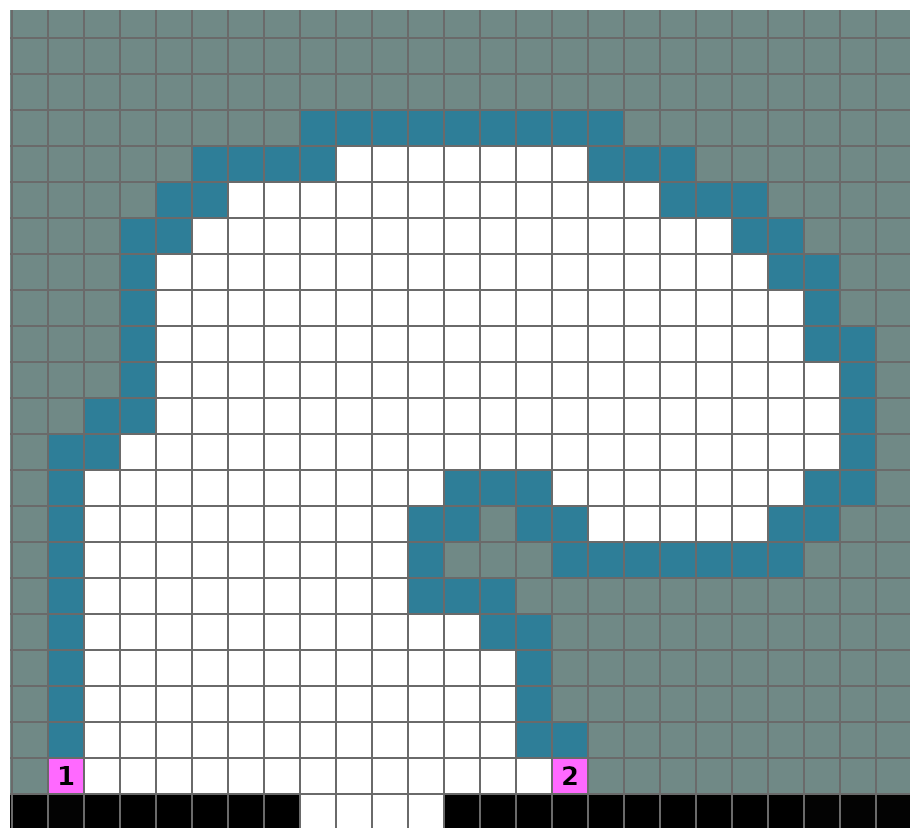
\includegraphics[clip=true, width=0.40\textwidth]{imagenes/ejemploSimpCub/a2.png}}
  \subfloat[Se elige un nuevo $\mli{fs}$ y se actualizan $\mli{UF}$, $\mli{FS_i}$ y $\mli{FP}$.]{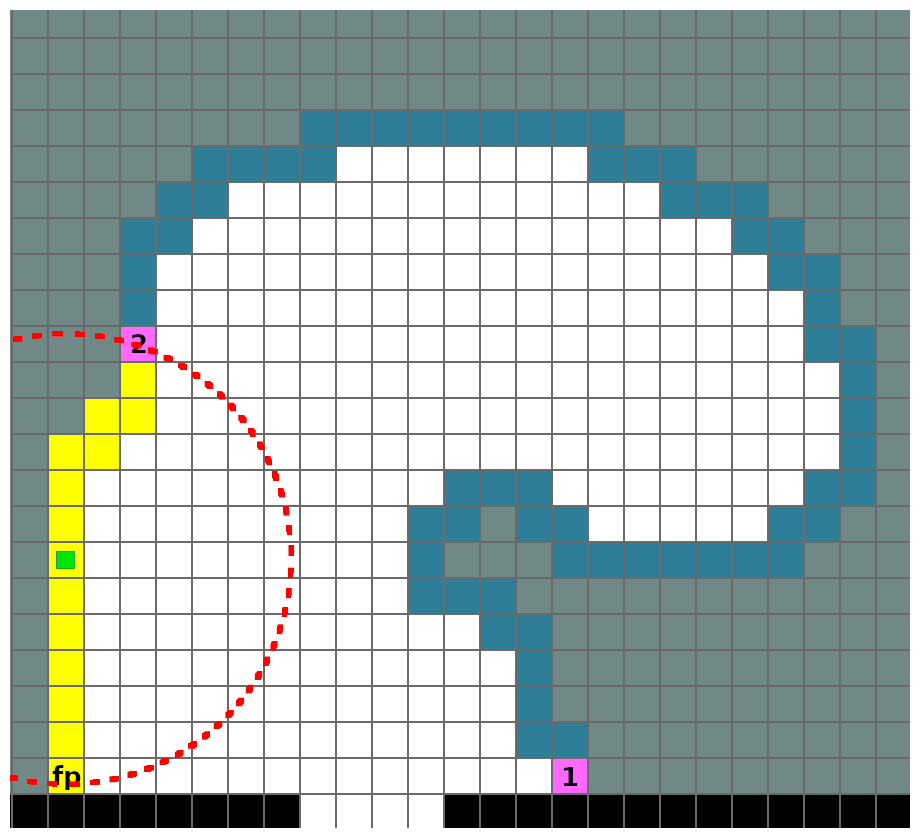
\includegraphics[clip=true, width=0.40\textwidth]{imagenes/ejemploSimpCub/b5.png}}
  \subfloat[Se elige un nuevo $\mli{fs}$ y se actualizan $\mli{UF}$, $\mli{FS_i}$ y $\mli{FP}$.]{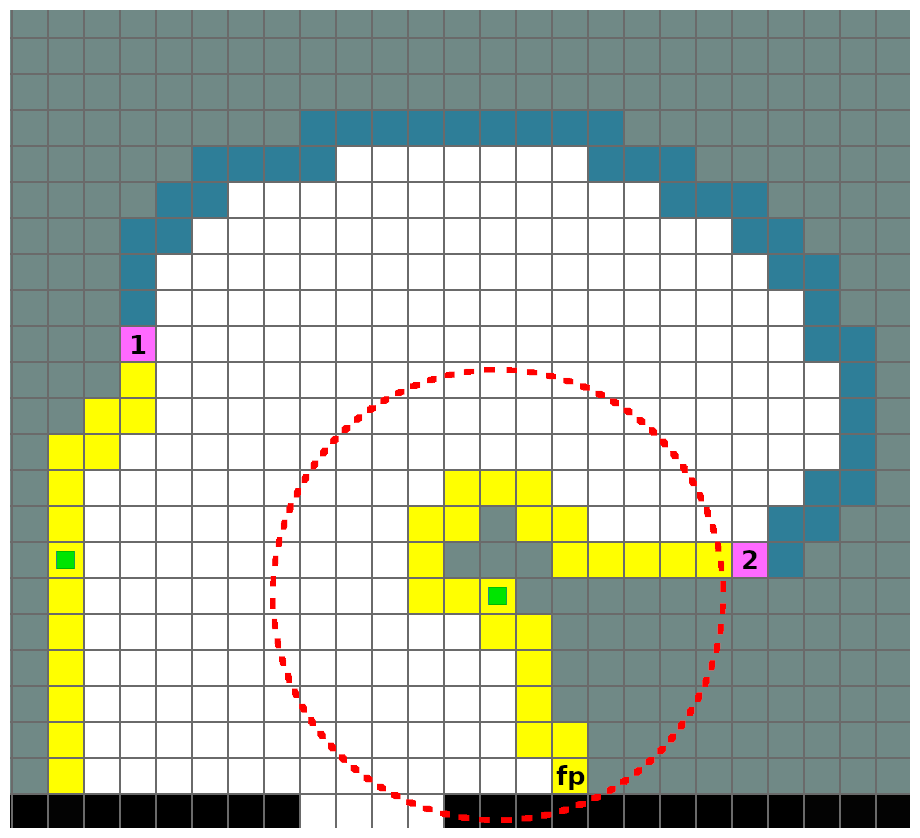
\includegraphics[clip=true, width=0.40\textwidth]{imagenes/ejemploSimpCub/c5.png}}

  \subfloat[Se elige un nuevo $\mli{fs}$ y se actualizan $\mli{UF}$, $\mli{FS_i}$ y $\mli{FP}$.]{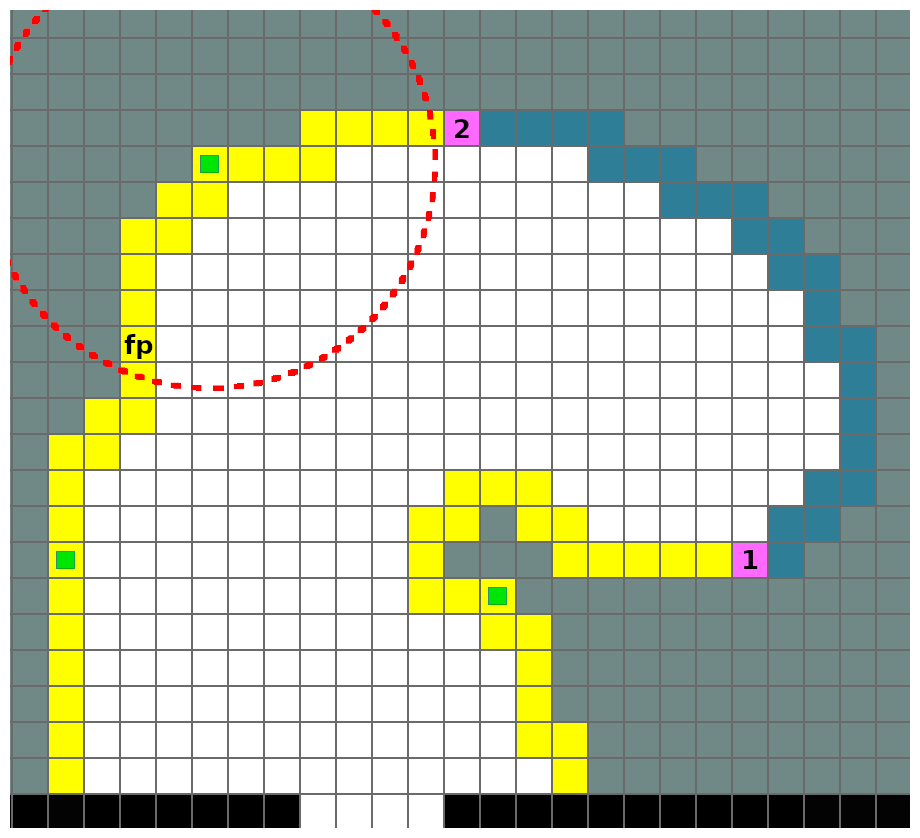
\includegraphics[clip=true, width=0.40\textwidth]{imagenes/ejemploSimpCub/d5.png}}
  \subfloat[Se elige un nuevo $\mli{fs}$ y se actualizan $\mli{UF}$, $\mli{FS_i}$ y $\mli{FP}$.]{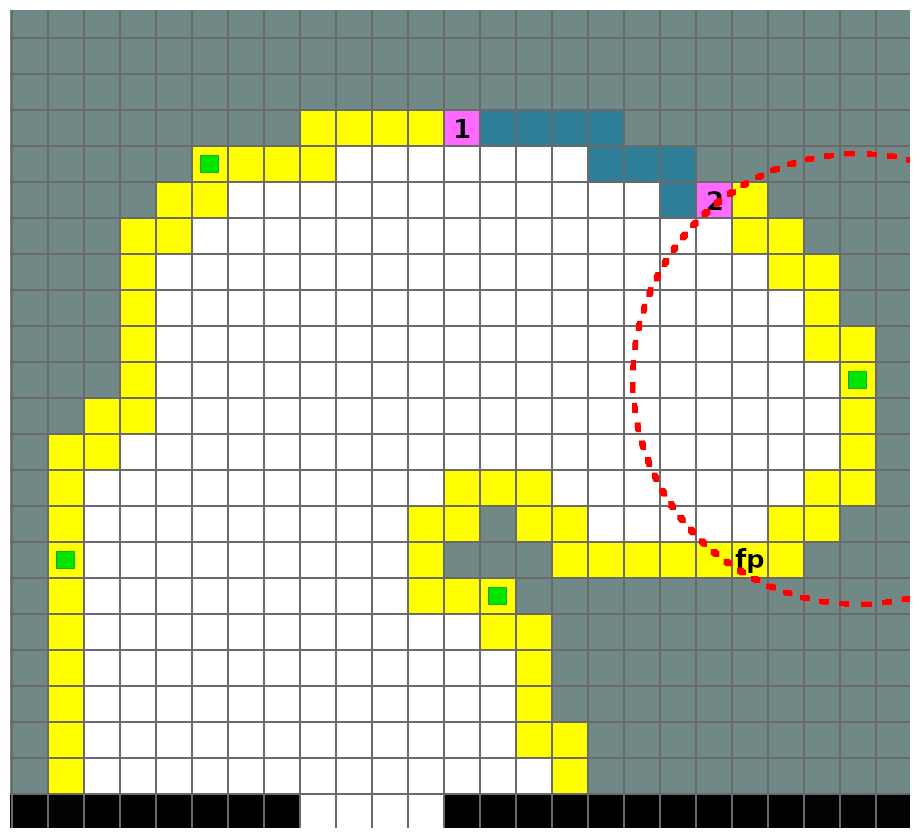
\includegraphics[clip=true, width=0.40\textwidth]{imagenes/ejemploSimpCub/e5.png}}
  \subfloat[Se elige un nuevo $\mli{fs}$ y se actualizan $\mli{UF}$, $\mli{FS_i}$ y $\mli{FP}$.]{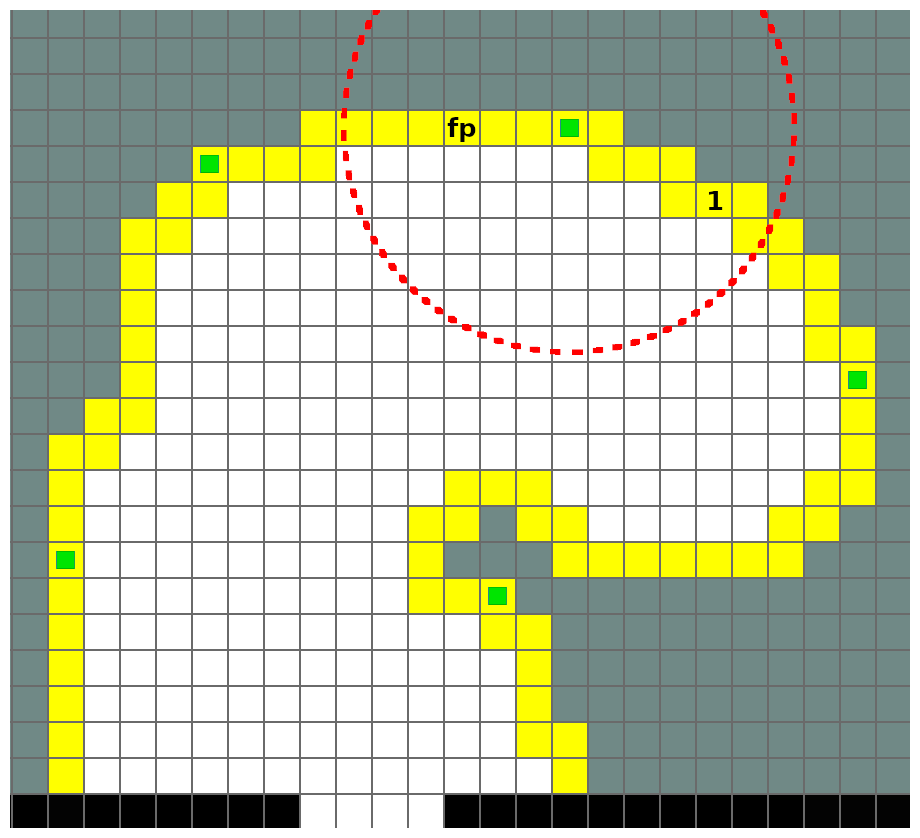
\includegraphics[clip=true, width=0.40\textwidth]{imagenes/ejemploSimpCub/f4.png}}

  \subfloat[$\mli{UF}=\emptyset$ por lo que el algorimo finaliza.]{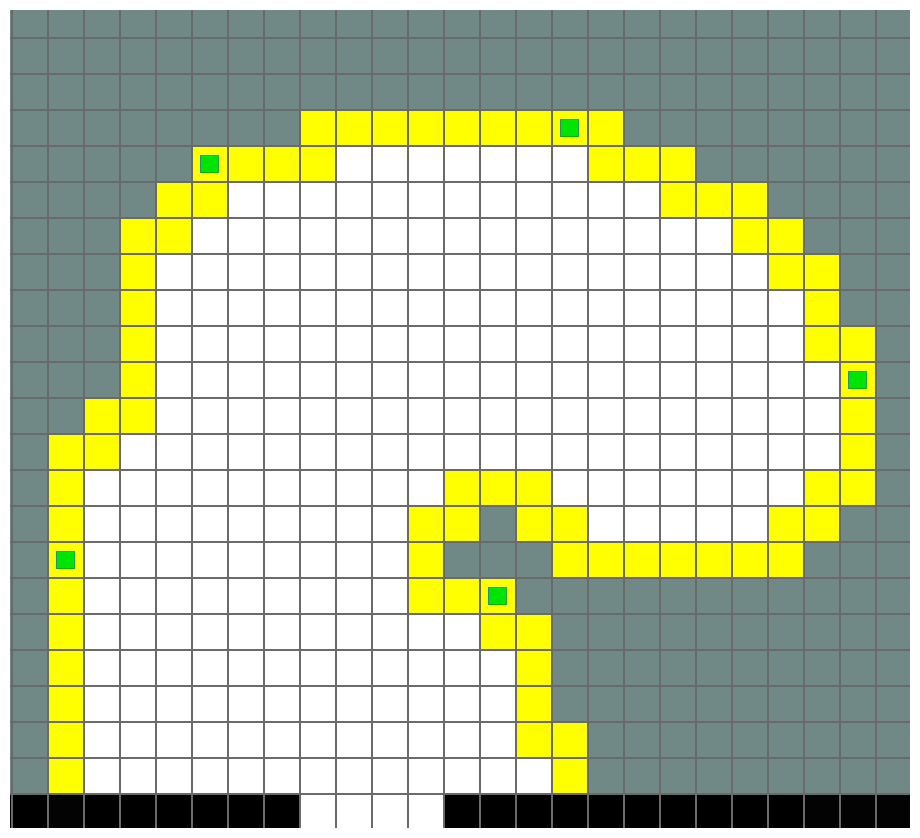
\includegraphics[clip=true, width=0.40\textwidth]{imagenes/ejemploSimpCub/zfinal1.png}}
  \subfloat[Resultado final.]{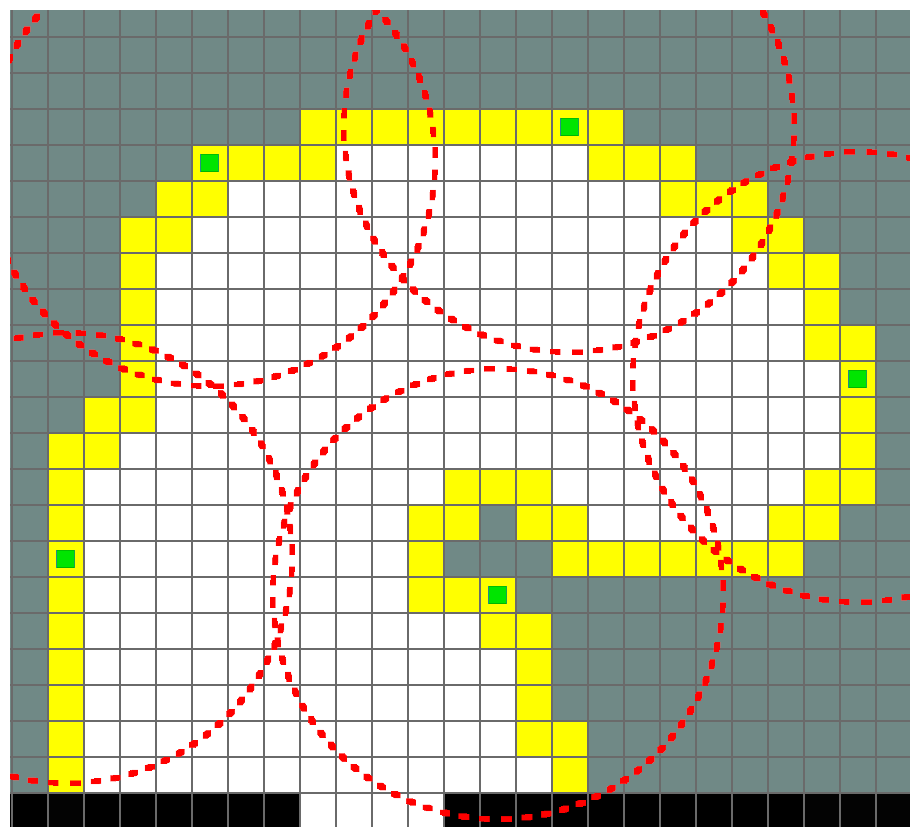
\includegraphics[clip=true, width=0.40\textwidth]{imagenes/ejemploSimpCub/zfinal2.png}}
  % \subfloat[$\mli{UF}=\emptyset$ por lo que el algorimo finaliza.]{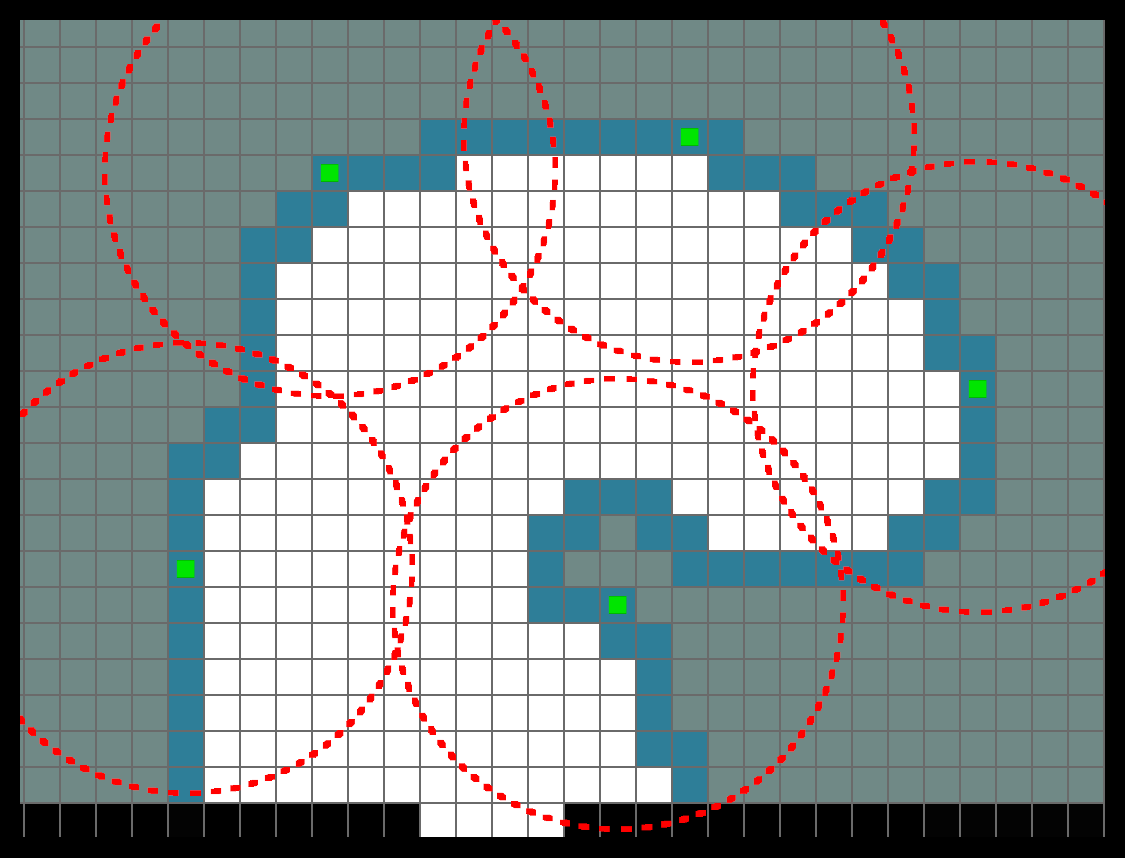
\includegraphics[clip=true, width=0.40\textwidth]{imagenes/ejemploSimpCub/zfinal3.png}}

  \caption[Proceso de simplificacion de fronteras según cubrimiento.]{Proceso
    de simplificacion de fronteras según cubrimiento.  Las fronteras de
    $F_i$ se indican con azul si pertenecen a $\mli{UF}$ y con amarillo de lo
    contrario. Con magenta se indican las celdas en $\mli{FP}$ siendo la
  numeracion su orden en la cola y $\mli{fp}$ la ultima desencolada. Las fronteras significativas se indican con
verde, siendo las circunferencias rojas de radio $rango=5.6$ (largos de celda) centradas en estas indicadores de su cubrimiento.}\label{fig:ejemploFSCub}

\end{figure}


\section{Asignación de tareas}
% Comentar el tema de que uso wurm, que cambio como obtengo el gvd haciendo uso de una variante del metodo inc presentado en Lau que tenia esas mejoras que se mencionaron en \ref{subsec:constGVDInc}. Decir que se va a comentar a detalle las variaciones desarrolladas la seccion \ref{sec:MiConstGVD}. 

Cuando un robot se encuentra ocioso este le solicita a la central que le asigne
una nueva tarea, esto desencadena un proceso de asignacion de
tareas que se describe a lo largo de esta seccion.

La asignación de objetivos se basa en la idea presentada en
\ref{subsec:wurmCoord}, que sostiene que es conveniente que los robots se
asignen a los objetivos de forma que estos se distribuyan uniformemente sobre
las habitaciones y corredores de un entorno estructurado, que se corresponden
las regiones (tambien llamados segmentos) de un mapa topológico (seccion
\ref{subsec:mapas}).

La asignación de objetivos consiste una subasta donde los objetivos de
exploracion son subastados entre los robots. La subasta se puede separar en
tres partes, \emph{obtencion de informacion}, \emph{valuacion} y
\emph{resolucion}. La \emph{obtencion de informacion}, es la etapa en la cual
todos los datos necesarios para llevar adelante la subasta (los objetivos de
exploracion) son determinados. La \emph{valuacion} abarca la distribuicion de
la informacion obtenida desde la central hacia los robots, el juicio de valor
de cada robot a cada objetivo recibido y el posterior envio de estas
valoraciones desde los robots hacia la central. La \emph{resolucion} contempla
la recepcion de las valoraciones por la central, un postprocesamiento sobre
estos, la asignacion de objetivos a robots segun la valoraciones y los
segmentos a los cuales pertenece cada objetivo, finalizando con la notificacion
del objetivo que le fue asignado a cada robot.

Con respecto a la separacion del problema de asignación de tareas mencionada en
la seccion \ref{sec:exploracion}, que establece dos partes, la identificacion
de objetivos y la asignación de objetivos; la primera forma parte de la
\emph{obtencion de informacion}, y la segunda se corresponde con el el resto de
lo que se describe en esta seccion.

% Para que la subasta sea llevada a cabo se deben distribuir los objetivos de
% exploracion entre los robots para que estos asignen valores a cada uno segun
% que tan conveniente les es llegar a ellos. Posteriormente los robots deben
% enviar las valuaciones realizadas a la central,

% la cual debera resolver que
% objetivo le corresponde a que robot segun las valuaciones recibidas y los
% segmentos en dode se ubican los objetivos, procurando distribuir lo mas posible
% a los robots sobre los segmentos. %, el metodo utlizado para lograr este se
% describe en \ref{subsec:MiResSub}. Finalmente la central notifica a cada robot
% su objetivo asignado.

% En resumen la subasta consiste en valuacion y resolucion. 
% valuacion: mandar los objetivos y esperar por sus valuiaciones.
% resolucion: resolucion y informar a laos robots

% asignación de objetivos se puede resumir en:
% \begin{enumerate}
%   \item Identificación de objtivos
% \end{enumerate}

% Para esto, una vez identificados los objetivos segun lo que se presenta en la
% sección \ref{subsec:MiSimp}, cada objetivo se le asigna la region que le
% corresponde en el mapa topológico contruido (seccion \ref{subsec:MiMapTOp}(

% \subsection{Mapa topológico}\label{subsec:MiMapTOp}


% \subsection{Protocolo de susbasta}\label{subsec:MiProtSub}
% Como se comentó anteriormente, la estación central es la encargada de la subasta de segmentos. Los robots son quienes recopilan la información, arman su mapa local y lo envían a la central, que por medio del modulo combinador de mapas, crea un mapa global. Este mapa global es convertido en una grilla de ocupación y segmentado a partr de un GVD. 
% Adicionalmente, fue reutilizada la implementación del algoritmo K-means para obtener las fronteras más significativas según el radio del robot, como fue explicado en al sección 2.1.

% Comentar proceso, enfasis en como es que funciona el flujo: pedido de los robots, identificacion, robots a valuar, recibir valuaciones, asignar y mandar asigaciones a los robots.

% Deternerse en cada parte explicando detalles.

% El pedido no es muy complejo.

% ID ya se explico.

% Envio es directo, la valuacion tiene algunos detalles.

% \subsubsection{Recepcion de valuaciones}
% Recepcion, aca esta el protocolo de recepcion, quizas es pertinente comentarlo por lo menos por arriba.
% \subsubsection{Envio de asignaciones}
% Mandar asignaciones es casi que trivial

\subsection{Obtencion de informacion}
Como se menciono todo comienza cuando un robot ocioso solicita un tarea a la
central, esto desencadana una nueva subasta de no encontrarse una en curso. Si
existe una en curso el robot recibira una tarea cuando esta termine, no es
necesario iniciar otra.

La etapa de \emph{obtencion informacion} es la primera etapa en llevase a cabo
al iniciarse la subasta. La informacion que se obtiene en esta son los
objetivos de exploracion, un GVD y las regiones del mapa mapa topológico del
entorno explorado que con el motivo de identificar en que segmento se encuentra
cada objetivo de exploracion, para porsteriomente poder asignar distribuyendo a
los robots sobre estos. 

La identificacion de objetivos se lleva a cabo con el metodo descrito en la
sección \ref{subsec:MiSimp}.

El mapa topológico se construye con la tecnica descrita en la seccion
\ref{subsec:mapaTopGVD} que se basa en el uso de un GVD. Uno de los cambios
principales con respecto al trabajo original de \cite{wurm2008coordinated} es
la forma en la cual se contruye el GVD. En el trabajo original se hace uso de
un metodo de construccion no incremental, en este proyecto con el motivo de
alcanzar una implementación que logre funcionar en tiempo real (seccion
\ref{subsec:constGVDInc}) se reemplaza por una variante del algoritmo
incremental \emph{brushfire dinamico} que se presentará en la seccion
\ref{sec:MiConstGVD}.


\subsection{Valuacion} \label{subsec:MiValSub}

Luego de obtenida la informacion se da comienzo a la estapa de \emph{valuacion}
distribuyendo dicha informacion desde la central hacia los robots. Cuando un
robot recibe la informacion este asigna dos valores a cada objetivo, el largo
del camino hacia a el y un costo asociado a la complejidad del camino.

Calcular el largo de un camino implica determnar el camino en sí. El camino se
calcula de forma distinta dependiendo de la clase de objetivo, existen dos,
triviales y no triviales.

Los objetivos triviales se definen como los objetivos para los cuales el
segmento de recta que existe entre el robot y el objetivo no contiene
obstaculos, de lo contrario el objetivo es no trivial. Para determniar esto, se
discretiza el segmento de recta en celdas \cite{foleyphillips} y se comprueba
en el mapa global (grilla de ocupacion) almacenado en el robot, alguna de las
celdas tiene un estado ocupado.

El camino en objetivos triviales se determina como dicho segmento de recta que
existe entre el robot y el objetivo, que se encuentra libre de obstaculos. 

En el caso de los objetivos no triviales se hace uso del GVD recibido como
parte de la informacion de la subasta, aprovechando que este constituye un
\emph{roadmap} (seccion \ref{subsec:mapacarr}). El GVD viene representado
como el conjunto de celdas que abarca, el proceso para construir el camino puede dividir 
en tres partes cada una asociada a una de las propiedades que caracterizan a un
\emph{roadmap}: accesibilidad, conectividad y capacidad de salida. La parte asociada
accesibilidad consiste en encontrar un camino desde el robot al GVD, lo cual se
hace a traves de un \emph{breadth-first search} (BFS), se comienza en la celda
asociada a la posicion del robot y se detiene apenas se visita una celda $c_1$
perteneciente al GVD. La que se relaciona con la capacidad de salida es analoga a la
accesibilidad pero el camino va desde el objetivo a alguna celda $c_2$ del GVD.
Por ultimo la parte vinculada con la conectividad se basa en establecer un
camino sobre las celdas del GVD desde $c_1$ a $c_2$, lo cual se hace aplicando
algoritmo $A^*$. Conectando esos tres caminos se obtiene el camnino completo.

El costo asociado a la complejidad en el caso de objetivos triviales se
determina como el tiempo estimado que demora el robot en rotar de forma que su
parte delantera apunte hacia el objetivo. Y en el caso de objetivos no
triviales se utiliza la maxima penalizacion usada para objetivos no triviales.
El proposito de esto es diferenciar los objetivos triviales sin beneficiar a
los objetivos no triviales. Este costo se aplica para incentivar a que el robot
ontinue siendo asignado a los objetivos triviales que tiene por adelante al
explorar.

Obtenidos ambos valores para cada objetivo estos se envian hacia la central
junto a la ubicacion actual del robot, siendo toda esta informacion en su
conjnto considerada una valuacion. \todo{o mensaje de valuacion, como quede mejor}

% De esta
% forma los objetivos triviales se valuan distinto segun que tanto tiene que
% rotar el robot para llegar a ellos y los objetivos no triviales tendran un
% costo no mayor al del peor objetivo no trivial.

% como el conjunto de celdas que abarca, el proceso para construir el camino es
% se puede dividir en encontrar tres subcaminos cada uno relacionado a una de las
% tres propiedades de un roadmap: accesibilidad, conectividad y capacidad de
% salida. La accesibilidad consiste en encontrar un camino desde el robot al GVD,

% La valuacion abarca la distribuicion de los objetivos de exploracion desde la
% central hacia los robots, la asignación de valores que cada robot debe hacer a
% cada objetivo y el posterior envio de estas valoraciones desde los robots hacia
% la central. 

\subsection{Resolución} \label{subsec:MiResSub}
% La resolucion es el proceso de asignar los objetivos La resolucion contempla
% la recepcion de las valoraciones por la central, la asignacion de objetivos a

% robots segun y la notificacion del objtivo asignado a los robots. 
% de exploracion a los
% robots. 
\subsubsection{Recepcion de valuaciones}
La resolucion comienza con la recepcion de las valuaciones realizadas por
los robots. Al recibirse la primera valuacion existe una ventana de tiempo en
la que la central continuara recibiendo nuevas valuaciones. Terminada esta
ventana se ejecuta un algormitmo que resulta en la asignacion de objetivos a
los robots.

El proposito de la ventana es que en escenarios reales los robots pueden dejar
de comunicarse por alguna razón (desconexiones de red, accidentes que dejen a
los robots sin funcionar, entre otros), por lo tanto esperar por las
valuaciones de todos los robots puede ser una espera infinita.

Dado que el problema que los robots deben resolver para generar las valoraciones es
similar, se asume que el tiempo se demora en generar las valoraciones tambien
es similar, adicionalemtente dicho tiempo es proporcional al area del
mapa que se encuentra explorada, por lo tanto se opto por utilizar una ventana
dinámica de un tamaño que, considerando lo que demoraron las valoraciones de
los robots en la subasta anterior, sea lo suficientemente grande como para que
todos los robots que esten en condiciones de responder con sus valoraciones
tengan el tiempo necesario para hacerlo.

Notar que una vez que se reciben las valoraciones de todos los robots
funcionales es innecesario continuar esperando, por lo tanto de recibirse
dichas valoraciones la ventana de resolución es terminada prematuramente
evitando esperas innecesarias.

Siendo $tr_i$ el tiempo que paso desde la recepcion de la primera valuacion
hasta el comienzo de la ejecucion del algormitmo de asignacion y $vr_i$ la
duracion de la ventana $i$ definida en \ref{eq:ventanaVals}.

\begin{equation} 
  vr_i = 
  \left \{ 
    \begin{aligned}
      0.5s                            \ \ \ \ \ \ \ \ & si\ i = 0\\ 
      max(0.5s + 2tr_{i-1}, vr_{i-1}) \ \ \ \ \ \ \ \ & si\ i > 0
    \end{aligned}
  \right .
  \label{eq:ventanaVals}
\end{equation}

El valor de la duracion $v_i$ resulta de asumir que de una subasta a la
siguiente no se demorara más del doble del tiempo en obtener las valuaciones de
todos los robots, dando un margen de error de 0.5 segundos, especialmente útil
cuando $rt_i$ es muy pequeño. Lo asumido se corresponde con lo ocurre en las
pruebas realizadas.

% por lo que sería contraproducente no esperar por la valoración de
% algún robot ya que dicha espera es mínima en comparación con lo que un robot
% debe esperar en caso de no ser considerado para la resolución.

% Para cumplir con el propósito propuesto se podría decir que la ventana sea de
% un tamaño muy grande o infinita, lo cual en un entorno simulado como el que se
% basa este trabajo no generaría problemas ya que los robots siempre pueden


% y como estas se guardan al recibirse
\subsubsection{Algoritmo de asignacion de objetivos}
% Segun lo explicado en la seccion anterior
Cuando la central recibe una valuacion de un robot $r_i$, esta se encarga de
procesar la informacion contenida en la valuacion de forma de obtener un unico
costo $c_{i,j}$ del robot $r_i$ a cada objetivo $o_j$. Para un objetivo en
$o_j$ la valuacion del robot $r_i$ contiene el costo $\mli{cca}_{i,j}$ del camino de
$r_i$ a $o_j$ y el costo $\mli{cco}_{i,j}$ asociado a la complejidad de dicho camino.
Adicionalmente a traves de la posicion recibida de $r_i$ se determina un descuento 
$\mli{dse}_{i,j}$ que toma un valor constante menor a cero ($-10$ en al
implemetnacion) si el robot $r_i$ pertence al mismo segmento que el objetivo
$o_j$ y cero de lo contrario. Finalmente el costo $c_{i,j}$ se calcula segun la
ecuacion \ref{eq:costoTot}.

\begin{equation} 
  c_{i,j} = \mli{cca}_{i,j} + \mli{cco}_{i,j} + \mli{dse}_{i,j}
  \label{eq:costoTot}
\end{equation}

Los costos $\mli{cca}_{i,j}$ y $\mli{cco}_{i,j}$ tienen como proposito
penalizar en la asignacion a los objetivos segun la dificicultad asociada a los
caminos que llevan a esto. Por otro lado el descuento $\mli{dse}_{i,j}$
incentiva que los robots se mantengan explorando un mismo segmento, lo cual
desencadena comportamientos deseables como el de que un robot continue
explorando un mismo corredor, revelando rapidamente la estructura de un entorno
estrucutrado.

% Los robots envian a la central dos valores junto a su posicion, cuando la central lo recibe estos se 

% esto, la posicion de dicho robot y
% dos valores, al recibirse la valuacion en la central dichos valores son
% procesados de forma

% La version original de \cite{wurm2008coordinated} lleva a cabo la asignacion
% utilizando el metodo hungaro. Este  
% de forma optima en $O(n^3)$ siendo $n$ el numero de tareas.

Con estos costos costos como insumos se ejecuta un algorimo de asignacion de
objetivos a robots, este tiene como proposito asignar objetivos a los robots de
que estos se distribuyan sobre los segmentos (seccion \ref{subsec:wurmCoord}).
\todo[inline]{El metodo hungaro capaz no considera que el numero de robots
  asigandos a un segmento debe ser menor que el numero de fronteras que tiene
  ya que no tiene sentido asignar a un robot a un segmento si este no tiene
  objetivos disponibles. Habria que ver bien como funciona el metodo hungaro,
  pero creo que es una asignacion robot-segmento que no considera otra cosa que
  el costo, num robots y num segmentos, por lo tanto el num de fronteras de un
  segmento no se estaria considerando.}

% El algorimo \ref{alg:resolucionsubastasegmentos} presenta un pseudocodigo del
% algormitmo de asigacion donde $R$ el conjunto de los identificadores de los
% robots, $O$ el conjnto de los identificadores de los objetivos y $Costos$ el
% conjunto los $c_{i,j}$ computados a partir de las valuaciones recibidas
El algorimo de asigacion, se corresponde al algorimo
\ref{alg:resolucionsubastasegmentos}, donde $R$ es el conjunto de los
identificadores de los robots de los cuales se recibieron valuaciones, $O$ el
conjnto de los identificadores de los objetivos valuados, $Costos$ un conjunto
de tuplas $(c_{i,j},r_i,o_j)$ los $c_{i,j}$ computados a partir de las
valuacion recibida de $r_i$ para $o_j$ y $S$ el conjunto de
segmentos. La funcion $segmento : O \rightarrow S$ dado un objetivo devulve el
segmento al que pertence y la funcion $\#objetivos : S \rightarrow N$ devuelve
el numero de objetivos en un segmento.
% Los conjuntos $O_1$,$O_2$,...,$O_k$,...,$O_{|S|}$ contienen los
% objetivos que estan dentro de un segmento $s_k\in S$.

\vspace{1cm}
  
\begin{algorithm}[H]
\SetAlgoLined
  \SetKwInOut{Input}{Entrada}
  \Input{$R, O, S, Costos$} % O_1, O_2,...,O_{|S|}$}
%   // PARTE 1
    $segObjs :=$ Multiconjunto vacio 

  
%   /// recorrida de todos los elementos del diccionario, con el propósito de construir segFrontColaPrio
    \ForEach{$s_k \in S $}{ 
     %ALT1 segObjs.encolar($|O_k|$)\\
     %ALT2 $segObj = segObj \cup \{|O_k|\}$\\
     $segObj = segObj \cup \{\#objetivos(s_k)\}$\\
    }
    
    $numSegs := |S|$\\
    $numRobs := |R|$\\
    $converge := false$\\

    \While{$\lnot (segObjs = \emptyset \lor converge$)}{
      $cocienteDist := numRobs\ \ div\ \ numSegs$\\
      $restoDist    := numRobs\ \ mod\ \ numSegs$\\
    
      $segObj := min\ segObjs$\\
      $segObjs := segObjs - segObj$\\
    
      $converge := (segObj > cocienteDist) \lor (restoDist = 0 \land segObj = cocienteDist)$\\
      \If{$\lnot converge$}{
        $numRobots := numRobots - segObj$\\
        $numSeg := numSeg - 1$\\
      }
    }
%   // PARTE 2
    $asignaciones := \emptyset$\\

    $segRobNums :=$ diccionario de $S$ a enteros, siendo 0 el entero asignado por defecto\\   

    \While{$R \neq \emptyset \land O \neq \emptyset$}{
      $(c_{i,j}, r_i, o_j) := min\ Costos$ \tcp{Tupla de $Costos$ con minimo $c_{i,j}$}
      $Costos := Costos - (c_{i,j}, r_i, o_j)$\\
      $s_k := segmento(o_j)$\\
      $distribuido := segRobNums[s_k] < cocienteDist \lor (restoDist > 0 \land segRobNums[s_k] < cocienteDist + 1)$\\
      \If{ $r_i \in R \land o_j \in O \land distribuido$ }{
        $asignaciones := asignaciones \cup (r_i,o_j)$\\
        $segRobNums[s_k] := segRobNums[s_k] + 1$\\
        $R := R - r_i$\\
        $O := O - o_j$\\
        \If{$segRobNums = cocienteDist + 1$}{
           $restoDist := restoDist - 1$\\
        }
      }
    }
  \Return asgnaciones 
    
 \caption{Asigacion de robots a objetivos}
 \label{alg:resolucionsubastasegmentos}
\end{algorithm}

El algorimo se puede dividir en dos partes, el \emph{calculo de valores}
$cocienteDist$, $restoDist$ (lineas 1-18) y la \emph{asignacion distribuida} (lineas
19-36). 

Los valores $cocienteDist$ y $restoDist$ se utlizan para lograr una asignacion
distribuida sobre los segmentos conisderando los objetivos contenidos en cada
uno. La distribucion deseada se corresponde con la distribucion que se logra al
hacer $N$ rondas en las que se asigna un solo robot por segmento con tenga
objetivos sin asignar. La ronda $N$ termina cuando no quedan robots o objetivos
por asignar. Si existen menos objetivos que robots se tiene que la ronda $N$
culmina con todos los objetivos asignados y algunos robots ociosos. De existir
mas objetivos que robots luego de la ronda $N$ se pueden tener segmentos cuyos
objetivos estan todos asignados y se tienen segmentos dentro de los que 
existen objetivos sin asignar, la distribucion sera unfirme sobre estos ultimos
segmentos. Es decir los $K$ segmentos que tienen objetivos sin asignar
cumpliran con (\ref{ec:uniform}), existiendo $restoDist$ segmentos con
$N=cocienteDist+1$ robots asignados y $K-restoDist$ segmentos con
$cocienteDist$ robots asignados. El \emph{calculo de valores} se lleva a cabo
inicializando $cocienteDist$ y $restoDist$ asumiendo una distribucion
completamente uniforme (lineas 5-6 y 9-10 primera iteracion), sin considerar si
es posible dado el numero de objetivos en cada segmento. Luego de forma
iterativa, segmento a segmento y comenzando por los que tienen menos objetivos
(lineas 11-12), comprobar si son de los segmentos cuyos objetivos seran todos
asignados (linea 13) y de serlo ajustar los valores para que la distribucion
sea uniforme en el resto de conjuntos (lineas 14-17 y 9-10). Las iteraciones
continuan hasta que solo quedan los segmentos en los que quedaran objetivos sin
asignar (linea 8), cuando esto sucede se dice que $cocienteDist$ y $restoDist$
convergen.
% a los valores consistentes con la distribucion deseada.

Con los valores $cocienteDist$ y $restoDist$ calculados la \emph{asignacion
distribuida} consiste en retirar las tuplas $(c_{i,j},r_i,o_j)$ de $Costos$
comenzando por las de menor costo $c_{i,j}$ (lineas 22-23) y para cada una de
estas asignar $r_i$ a $o_j$ (lineas 27-33), si $r_i$ y $o_j$ no forman parte de
ninguna de las asiganciones realizadas hasta el momento, y si la asignacion
mantiene la distribuicion deseada (lineas 25-26). Esto se repite hasta que
todos los robots estan asignados o que no quedan mas objetivos por asignar
(linea 21).

% , estos se calculan de forma que todos los segmentos tengan todos sus objetivos asignados a robots, un numero de robots asignadosk

En resumen, la central asigna a los robots a objetivos considerando los costos
de forma voraz y con la restriccion de distribuir los robots sobre los
segmentos considerando la cantidad de objetivos que contienen. Luego de
ejecutar el algorimo de asigacion la central informa a cada robot el objetivo
que le fue asignado, quedando a la espera de nuevos pedidos por parte de los
robots para comenzar una nueva subasta. 


\section{Construccion del GVD}\label{sec:MiConstGVD}

Considerando los problemas de eficiencia del algorimo \emph{brushfire} (seccion
\ref{subsec:constGVD}) y los problemas de su version incremental
\emph{brushfire dinamico} (seccion \ref{subsec:constGVDInc}) como fue propuesta
originalmente en \cite{kalra2009incremental}, se decidio basar la construccion
del GVD en la version de \emph{brushfire dinamico} propuesta en \cite{Lau2013},
a la que se estara haciendo refencia al mencionar \emph{brushfire dinamico}
desde este punto.

Dado que se segmenta el entorno segun el metodo que se comenta en la seccion
\ref{subsec:mapaTopGVD}, se es necesario encontrar los puntos criticos y lineas
criticas asociadas al GVD construido. Mientras que entcontrar los puntos
criticos (celdas criticas en el contexto de la implemtacion) solo requiere de
las celdas pertenecientes al GVD y el del mapa de distancias subproducto de
\emph{brushfire dinamico}, las lineas criticas requieren de encontrar las
celdas mas cercanas de los generadores que generan la pertenecia de la celda
critica al GVD (a los que se denominará como celdas base), informacion no
es un resultado de \emph{brushfire dinamico}. En \emph{brushfire dinamico} no
se manejan los generadores base de foma directa, la pertenencia de una celda al
GVD se determina segun si las celdas ocupadas mas cercanas $oc_1$ y $oc_2$ de
las dos celdas $c_1$ y $c_2$ involucradas en un choque de olas son o no
adyacentes entre si. De esta forma se logra aproximar el GVD resultante de
considerar generadores conexos y convexos \ref{subsec:GVD}. Determinar los
puntos base con este metodo no es posible ya que una vez determinada la
pertenecia de una celda $c_1$ al GVD no se almacena 


Se mantienen todos los obts a minima distancia, y los que \say{casi} estan a
minima distancia, siendo estos los puntos bases (puntos mas cercanos a
generadosres base) tomados en cuenta, segun estos se define si un punto pertenece o no al GVD.

Aunque existe una etapa de erosion posterior como en Lau para asegurar la sparceness. Comentar que se basa en el A de zhang, que en principio es mas eficiente que chequear patrones

Oportunidad de comentar que mejora sobre lau porque perminte generar gvd en
lugares a dist 1 de los obstaculos, cosa que lau no permite ni explica porque.

Desribir problemas de desconexion presentados en las diversas implementaciones: 
\begin{itemize}
  \item mencionar los de kalra
  \item los generados por considerar dist 1 en lau
  \item y mostrar que liu ming aunque no explique que hace bien tambien los tiene?
\end{itemize}

\subsection{Consideraciones sobre el espacio desconocido}
Explicar el problema de considerar lo desconocido, como no hacerlo lleva a GVD
disconexos, explicar lo qeu se encuentra en el estado del arte (explicar como
esta aplica para entornos abiertos), la alternativa de que los bordes no sean
obstaculos (como esta no aplica a entornos abiertos y genera mas costos) y la
alternativa de que las fronteras sean emisoras de GVD y lo desconocido no sea
atravezable por las ondas y porque esto implica mucho menos costos para mapas
cuando estos se comienzan a explorar y se componen de muchas celdas
desconocidas.

% \subsection{Segmentacion}
% yo diria de 

% Creo que aca en realidad no habria que comentar mucho si es que hay que comentar, son las mismasideas que las comentadas en \ref{subsec:mapaTopGVD}.

% Quizas mencionar que se usa la descomposicion en componentes conexas y como. 

% Mencionar el uso de sources y pseudosources para hacer lineas criticas. Discretizacion de lineas?

% Algunos resultados?

\section{Planificación}
Describier el proceso a detalle desde que llega un camino, y como este se va
completando poco a poco hasta llegar al objetivo de exploracion al final del
camino.

Tocar por arriba los mecanismos de recuperacion si queda facil.

\section{Construcción cooperativa del mapa}
Aca tengo que comentar como funcina el map merger:

las actualizaciones, que las da el stack de navegacion, lo que esto implica, que incrementales (solo porcion del mapa) 

Y por otro lado ocmo estas actualizaciones se integra (el metodo que se describe en \cite{stachniss2009robotic}).

% basura de: \subsection{Simplificacion de fronteras basada en cubrimiento}

 %  \item Actualizar $\mli{FS_i}$ agregando $\mli{fs}$:

 %    $\mli{FS_i} := \mli{FS_i} \cup \{\mli{fs}\}$

 %  \item Actualizar $\mli{UF}$ removiendo todas las fronteras cubiertas por $\mli{fs}$:

 %    $\mli{UF} := \mli{UF} - \mli{RC}$

 %    Con $\mli{RC}=\{ f\in F_i : d_{\mli{fs}}(f) \leq rango\}$ las celdas recien
 %    cubiertas.

 %  \item Si $\mli{UF} \neq \emptyset$ volver a 1. de lo contrario devolver $FS_i$.
% \end{enumerate}



% Adicionalmente, se simepre que sea menor a $rango$ se usara la heuristica de 



% eleccion de
% $\mli{fs}$ debe considerar el resto de fronteras por cubrir y su cercania a los
% obtaculos, por ejemplo si $\mli{UF}$ es tan pequeño como para que se cubra
% completamente con una unica frontera significativa $\mli{fs}$ esta se deberia
% elegir para que este centrada en $\mli{UF}$.
%%acatoy
% Se asume que las fornteras mas centradas se encuentran a una
% distancia $dCen = max\{ d_{\mli{PF}}(\mli{f}) : f\in\mli{UF} \}/2$ de
% $\mli{fp}$. 

% Combiando ambos factores se determina que el conjunto de fronteras
% significativas candidatas 

 % puede resumir como elegir una frontera $\mli{fs}$ que
% cubra 

% comienza desencolando una frontera $\mli{fp}$ de $\mli{FP}$
% que debe no estar cubierta todavia, por lo cual de estar cubierta se descarta y
% se vuelve a desencolar. 


% , si dicha forntera ya esta cubierta la eleccion se cancela 
% \begin{enumerate}
 %  \item 
 %  \item Actualizar $\mli{FS_i}$ agregando $\mli{fs}$:

 %    $\mli{FS_i} := \mli{FS_i} \cup \{\mli{fs}\}$

 %  \item Actualizar $\mli{UF}$ removiendo todas las fronteras cubiertas por $\mli{fs}$:

 %    $\mli{UF} := \mli{UF} - \mli{RC}$

 %    Con $\mli{RC}=\{ f\in F_i : d_{\mli{fs}}(f) \leq rango\}$ las celdas recien
 %    cubiertas.

 %  \item Si $\mli{UF} \neq \emptyset$ volver a 1. de lo contrario devolver $FS_i$.
% \end{enumerate}

%%%%%%%%%%%%%%%%%%%%%%%%%%%%%%%%%%%%%%%%%%%%%%%%%%%%%%%%%%%%%%%%%%%%%%%%%%%%%%%%%%%%%

% De los pasos presentados el primero es el principal y tambien el mas complejo
% del algorimo.

% Los pasos del 2 al 4 no presentan ambigüedad, siendo el paso 1 en el que resta
% aclarar, especificamente lo que resta aclarar es el criterio con el que se
% elige la frontera significativa. La eleccion en un principio podria ser
% aleatoria y el algormitmo daria resultados validos, pero esto dejaria a la
% suerte la calidad de la solucion. La idea seria elegir de forma determinista a
% una frontera significativa buscando que cubra la mayor cantidad de frotneras
% mientras se evita cubrir nuevamente fronteras que ya sean cubiertas por otra
% frotntera significativa. 

% La tecnica desarrollada se basa en mantener una cola FIFO en donde se guardaran
% los proximas fronteras a cubrir $\mli{PF}$, 
% El proceso para elegir una nueva forntera significativa $\mli{fs}$ consiste en
% desencolar una frontera $\mli{PF}$ de $\mli{PF}$ para posteriomente determinar
% el conjunto de fronteras significativas candidatas $\mli{FSC}$ como las
% fronteras sin cubrir desde las cuales se cubre a $\mli{PF}$ estando lo mas
% alejadas posible de esta, es decir, que $\mli{FSC}$ %$= \{f\in \mli{UF} : d_{\mli{fs}}(\mli{PF})= rango$\}
% sera el conjunto de celdas en $\mli{UF}$ que solapen con la circunferencia del
% circulo de radio $rango$ centrada en $\mli{PF}$ denotada como $\mathscr{C}(\mli{PF},rango)$.
% Para elegir una nueva frontera significativa $\mli{fs}$ se debe elegir una
% frontera de $\mli{FSC}$, que en esta propuesta se hace de forma arbitraria.


% Ahora resta tratar dos casos bordes, el primero es la inicializacion de
% $\mli{PF}$ cuando no existen fronteras adyacentes a obstaculos, cuando esto
% sucede para inciar el algorimo basta con agregar una unica frontera arbitraria
% de $F_i$ a $\mli{PF}$. El otro caso es el que se presenta si $\mli{FSC} = \emptyset$
% \todo{esto esta mal, en realidad esta mal desde antes cuando se presenta FSC, FSC busca que las candidatas queden centradas. Por lo que el radio puede ser menor al rango aunque haya una (o mas) celda solapada conla circunferencia de radio rango}
% , es
% decir la circunferencia del circulo de radio $rango$ centrada en $\mli{PF}$ no
% se solapa con ninguna celdas en $\mli{UF}$. Cuando esto sucede lo que se hace
% es reducir el radio del circulo a $\frac{max\{ d_{\mli{PF}}(\mli{f}) :
% f\in\mli{UF} \}}{2}$ la divicion entre dos busca que la circunferencia se
% solape sobre el punto medio entre $\mli{PF}$  y la celda de $\mli{UF}$ mas
% alejada de $\mli{PF}$, quedando la nueva frontera significativa centrada
% (figura ejemplo de esto).

% Para que el criterio de eleccion propuesto funcione de forma correcta es
% necesario agregar al paso 2 que  se deben encolar a $\mli{PF}$ todas las
% fronteras del siguiente conjunto $\{ f \in \mli{UF} : \exists c \in \mli{FS_i}
% - \mli{UF}, f \in ady(c)\}$ que no esten ya encoladas.

% $\mil{CF}$ de las fronteras
% cubiertas pos la nueva $\mli{fs}$, encolan a $\mil{PF}$ a las celdas de $


% elegir
% $\mli{fs}$ como uno de las 

% La condicion de distancia busca maximizar la
% cantidad de fronteras que cubre la nueva frontera significativa.

% EL algorimo se basa en la idea de que una buena distribucion de fronteras
% significativas deberia mantener en su mayor parte una distancia de $rango*2$
% entre cada frontera significativa, ya que esta es la distancia maxima que se
% puede tener para asegurar qu se cumpla el cubrimiento. 
